\chapter{RESULT AND DISCUSSION}
\label{sec:chap4_result}
% Please add the following required packages to your document preamble:
% \usepackage{multirow}
% \usepackage[table,xcdraw]{xcolor}
% If you use beamer only pass "xcolor=table" option, i.e. \documentclass[xcolor=table]{beamer}
\section{PhysioExercise Dataset}
\label{sec4:dataset_evaluation}
This section is about the collected dataset and its details. Our dataset consists of 9 classes according to the predefined elderly exercise activities. Within each class, videos were taken as described in Methodology. We take several physical issues that are common in the elderly. There are three categories of physical issues that we take for this dataset, i.e., frozen shoulder, tennis elbow, and knee pain. In brief, frozen shoulder is a common condition affecting the elderly, characterized by pain and limited movement in the shoulder joint. The second physical problem is tennis elbow. Tennis elbow is a condition characterized by pain and tenderness on the outside of the elbow. The knee as the main support of the body often experiences knee pain problems.
% Bagian ini menjelaskan dataset yang telah dikumpulkan dan rinciannya. Dataset kami terdiri atas 9 kelas sesuai dengan aktivitas latihan elderly yang ditentukan sebelumnya. Dalam setiap kelasnya, video diambil berdasarkan yang telah dijelaskan pada bagian XX. Kami mengambil beberapa masalah fisik yang awam terjadi pada elderly. Terdapat tiga kategori masalah fisik yang kami ambil untuk dataset kali ini, yaitu frozen shoulder, tennis elbow, dan knee pain. Secara singkat, frozen shoulder adalah kondisi umum yang mempengaruhi elderly, ditandai dengan nyeri dan gerakan terbatas pada sendi bahu. Masalah fisik yang kedua adalah tennis elbow. Tennis elbow adalah kondisi yang ditandai dengan rasa nyeri dan nyeri tekan pada bagian luar siku. Adapun lutut sebagai penopang utama badan seringkali mengalami masalah knee pain.

\begin{table}[h!]
	\caption{Physiotherapy exercises used as dataset classes and the distributions.}
	\label{tab:class-dataset}
	\centering
	\begin{tabularx}{\textwidth}{|l|X|r|r|}
		\hline
		\textbf{Physical Issue}                            & \textbf{Physiotherapy \newline Exercise} & \textbf{Total Person} & \textbf{Total Video} \\ \hline
		\multirow{4}{*}{Frozen Shoulder}
		                                                   & Adduction \newline Abduction             & 5                     & 206                  \\ \cline{2-4}
		                                                   & Left Arm \newline Circumduction          & 5                     & 227                  \\ \cline{2-4}
		                                                   & Right Arm \newline Circumduction         & 6                     & 227                  \\ \cline{2-4}
		                                                   & Shoulder Flexion \newline Tension        & 7                     & 229                  \\ \hline
		Tennis Elbow                                       & Elbow Flexion \newline Tension           & 5                     & 219                  \\ \hline
		\multirow{4}{*}{Knee Pain}
		                                                   & Left Knee Flexion \newline Extension     & 5                     & 195                  \\ \cline{2-4}
		                                                   & Right Knee Flexion \newline Extension    & 5                     & 195                  \\ \cline{2-4}
		                                                   & Left Leg Flexion \newline Extension      & 5                     & 206                  \\ \cline{2-4}
		                                                   & Right Leg Flexion \newline Extension     & 5                     & 195                  \\ \hline
		\multicolumn{3}{|l|}{\textbf{Total video dataset}} & 1899                                                                                    \\ \hline
	\end{tabularx}
\end{table}

Based on the three physical issues of the elderly that have been mentioned, we determine the exercise activities. Table \ref{tab:class-dataset} shows the exercise activity classes used in this work. There are a total of 9 kinds of activities performed to solve the above physical issues. There are 4 kinds of exercises to prevent frozen shoulder problems. The activities are adduction abduction, left arm circumduction, right arm circumduction, and shoulder flexion tension. These four exercises are movements that use the shoulder as the main focus in doing them. We take one exercise activity to prevent tennis elbow problems, which is elbow flexion tension. This movement uses the arm as the main focus. Finally, there are 4 types of training activities to prevent knee pain problems. The training activities are left knee flexion extension, right knee flexion extension, left leg flexion extension, and right leg flexion extension. Left knee flexion extension and right knee flexion extension are movements performed in a sitting position with the thighs and calves forming a \ang{90}. In this movement an elderly person will try to straighten their calves forward. The left leg flexion extension and right leg flexion extension are performed in a standing position. An elderly person will try to bend their knees backwards so that the thighs and knees form a \ang{90} angle.
% Dari tiga masalah fisik elderly yang telah disebutkan, aktifitas latihan kami tentukan. Tabel 1 menunjukkan kelas aktifitas latihan yang digunakan pada pekerjaan ini. Total terdapat 9 macam aktifitas yang dilakukan untuk penyelesaian permasalahan fisik di atas. Terdapat 4 macam latihan untuk mencegah permasalahan frozen shoulder. Aktifitas yang dimaksud adalah adduction abduction, left arm circumduction, right arm circumduction, dan shoulder flexion tension. Keempat latihan ini merupakan gerakan yang menggunakan bahu sebagai tumpuan utama dalam melakukannya. Kami mengambil satu aktifitas latihan untuk mencegah masalah tennis elbow, yaitu elbow flexion tension. Gerakan ini menggunakan lengan sebagai tumpuan utama. Terakhir, terdapat 4 jenis aktifitas latihan untuk mencegah permasalahan knee pain. Aktifitas latiha yang dilakukan adalah left knee flexion extension, right knee flexion extension, left leg flexion extension, dan right leg flexion extension. Left knee flexion extension dan right knee flexion extension merupakan gerakan yang dilakukan dalam posisi duduk dengan paha dan betis membentuk sudut \ang{90}. Pada gerakan ini seorang elderly akan berusaha untuk meluruskan betisnya ke depan. Adapun left leg flexion extension dan right leg flexion extension dilakukan dalam posisi berdiri. Seorang elderly akan berusaha menekuk lututnya ke belakang sehingga paha dan lutut membentuk sudut \ang{90}.

\begin{figure}[h!]
	\centering
	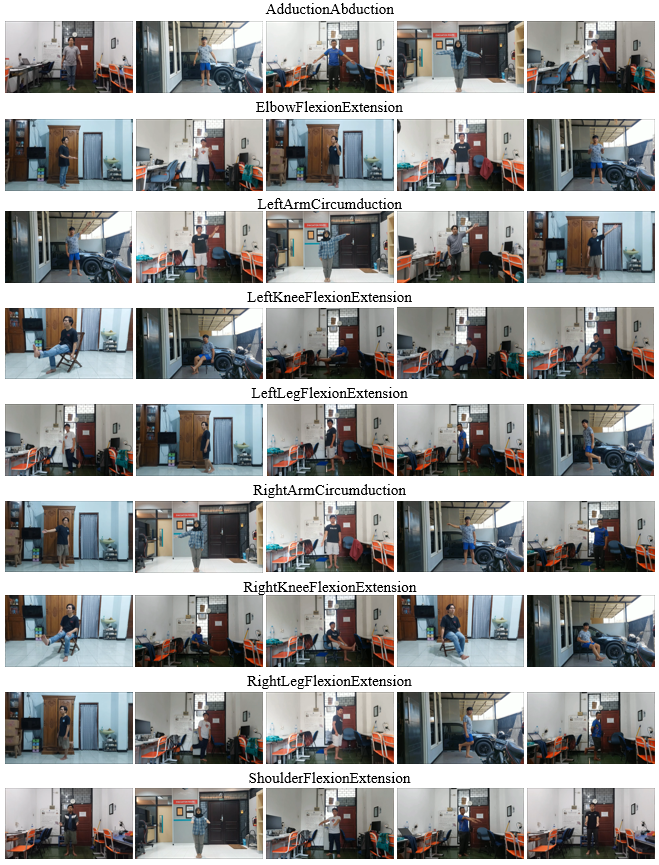
\includegraphics[width=1\textwidth]{bab4/ar_DatasetDist.png}
	\caption{Dataset distribution of PhysioExercise.}
	\label{fig:DatasetDistribution}
\end{figure}

We used multiple subjects to conduct the data acquisition process. There were at least 7 different subjects for this data acquisition process. The age range of the subjects in this work is between 21 to 36 years old. A wide age range was chosen because the feature used for training is pose estimation keypoint extraction. Moreover, these subjects are in good health, which makes it easier to capture the right movements in accordance with the physiotherapist's recommendations. There are a total of 1899 videos in this dataset.
% Kami menggunakan beberapa subjek untuk melakukan proses akuisisi data. Terdapat setidaknya 7 subjek berbeda untuk proses akuisisi data ini. Rentang usia subjek pada pekerjaan ini antara usia 21 hingga 36 tahun. Rentang usia yang beragam dipilih karena fitur yang digunakan untuk pelatihan adalah ekstraksi keypoint estimasi pose. Moreover, subjek-subjek ini dalam kondisi sehat, sehingga memudahkan dalam pengambilan gerakan yang tepat dan sesuai dengan anjuran physiotherapist. Total terdapat 1899 video pada dataset ini.

Figure \ref{fig:DatasetDistribution} shows the diversity and distribution of the dataset for each class. The dataset is organized to have a variety of capture angles, such as front view, left view, and right view. The capture angle for each view was varied to close to a \ang{90} relative to the front view. In addition, the video illumination level was also varied. We took the dataset in several time situations, such as morning, afternoon, evening, and night. Some videos have normal light and others have low light. The diverse lighting is intended to make the model adaptable to various lighting conditions. We took this dataset in several different environments, namely a laboratory environment and a home environment. The home environment was chosen to match the use of the model that will be used by the elderly in their respective homes.
% Gambar XX menunjukkan diversitas dan distribusi dari dataset untuk setiap kelasnya. Dataset diatur agar memiliki variasi sudut pengambilan, seperti front view, left view, dan right view. Sudut pengambilan untuk masing-masing pandangan dibuat beragam hingga mendekati sudut 90 relatif terhadap front view. Selain itu, tingkat penerangan video juga beragam. Kami mengambil dataset dalam beberapa situasi waktu, seperti pagi hari, siang hari, sore hari, dan malam hari. Sebagian video memiliki normal light dan sebagian sisanya memiliki low light. Pencahayaan yang beragam ditujukkan agar model yang dihasilkan dapat beradaptasi untuk berbagai kondisi penerangan. Kami mengambil dataset ini dalam beberapa macam lingkungan, yaitu lingkungan laboratorium dan lingkungan rumah. Macam lingkungan rumah dipilih untuk menyesuaikan dengan penggunaan model yang akan digunakan oleh elderly di rumah masing-masing.


% Setiap kelasnya memiliki data sebanyak 150 video. Sejak pemanfaatan keypoints sebagai fitur dalam pelatihan, video-video tersebut harus dipotong menjadi urutan-urutan citra yang merepresentasikan aktivitas latihan elderly. Dataset kami saat ini memiliki keragaman durasi video mulai dari 5 - 16 detik. Satu video kami convert menjadi urutan-urutan citra sebanyak 250 citra. Kami membagi sebuah video menjadi 250 frame secara merata dari awal frame hingga akhir frame agar merepresentasikan urutan aktivitas latihan elderly. Sejak setiap estimasi pose memiliki 33 keypoints dan 150 data setiap kelasnya, total keypoint yang diekstraksi setiap kelasnya sebesar 1350 keypoints. Total keseluruhan keypoints yang diekstrak untuk 9 kelas adalah 44500. 

\section{Video Frame Extraction}
\label{se4:VIdeoExtraction}

\begin{figure}[h!]
	\centering
	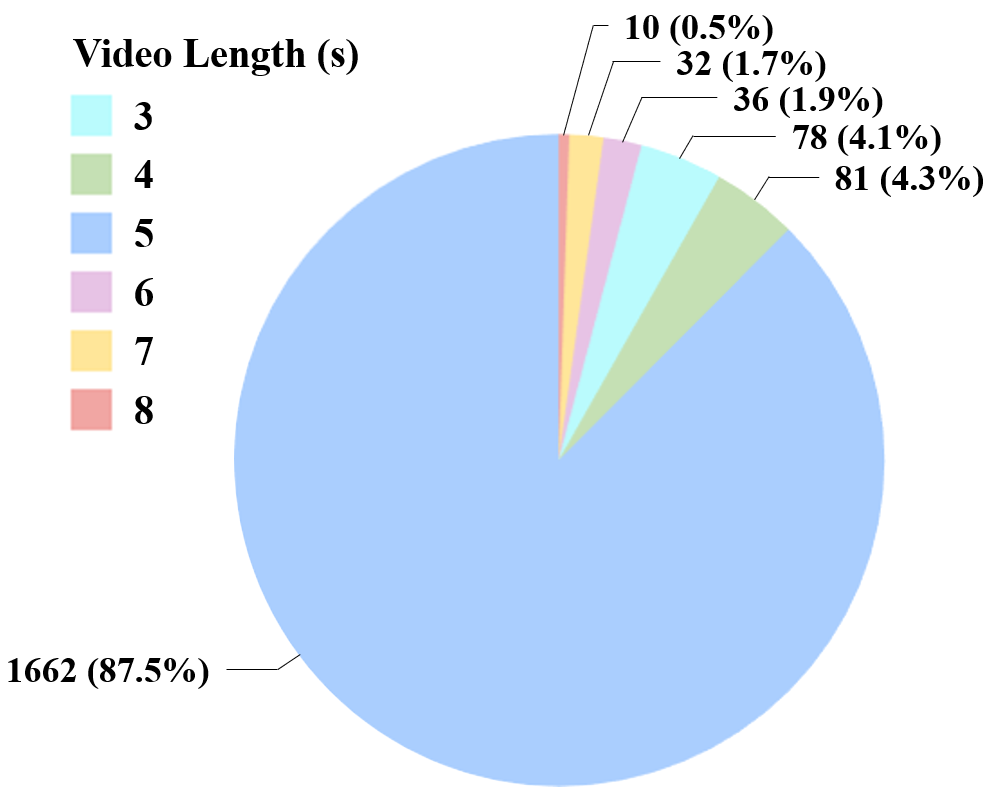
\includegraphics[width=0.6\textwidth]{bab4/ar_VideoLength.png}
	\caption{Statistics for the length distribution of our video dataset. Videos with a length of 5 seconds are the most recorded.}
	\label{fig:VideoLengthDistribution}
\end{figure}

The acquired dataset is a set of exercise activity videos for the elderly. Since the Mediapipe framework performs frame by frame pose estimation, our data must first go through a video frame extraction process. The video data we have is a short duration video. Figure \ref{fig:VideoLengthDistribution} shows the distribution of video length in the dataset. The duration of the videos we collected is in the range of 3 to 8 seconds. The duration with the least amount of data is 3 seconds, with only a total of 10 videos or 0.5\% of the overall data. In contrast, the duration with the most data is 5 seconds, with a total of 1662 videos or 87.5\% of the overall data.
% Dataset yang telah diakuisisi adalah sekumpulan video aktifitas latihan untuk elderly. Sejak framework Mediapipe melakukan estimasi pose frame by frame, data yang kami miliki harus melalui proses video frame extraction terlebih dahulu. Data video yang kami miliki merupakan video dengan durasi yang pendek. Gambar \ref{fig:VideoLengthDistribution} menunjukkan pesebaran panjang video pada dataset. Durasi dari video yang kami kumpulkan berada pada rentang 3 hingga 8 detik. Durasi dengan jumlah data paling sedikit adalah 3 detik, dengan hanya total 10 video saja atau 0.5\% dari keseluruhan data. Sebaliknya, Durasi dengan jumlah data paling banyak adalah 5 detik, dengan total 1662 video atau 87.5\% dari keseluruhan data.

Video frame extraction is done by dividing each video into 100 frames. This number of frames is determined so that not too many frames are extracted (12 - 30 FPS). We extract the video into fewer frames because we want to avoid frames that have too much motion blur. Motion blur in the context of pose estimation can blur the information carried, resulting in frames that are not good for deep learning training data. On the other hand, we also keep the overall information in a video intact. Within the 100 frames for a video, we spread them evenly throughout the video from beginning to end. So no information is left out in this video frame extraction.
% Video frame extraction dilakukan dengan membagi setiap video menjadi 100 frames. Jumlah frame ini ditentukan agar tidak terlalu banyak frame yang diekstrak (1 - 5 FPS). Kami mengekstrak video menjadi lebih sedikit frame karena kami ingin menghindari frame yang memiliki terlalu banyak motion blur. Motion blur dalam konteks estimasi pose dapat membuat informasi yang dibawa menjadi kabur, mengakibatkan frame yang tidak bagus untuk menjadi data pelatihan deep learning. Di lain sisi, kami juga tetap menjaga keseluruhan informasi dalam satu video tetap utuh. Dalam 100 frames untuk sebuah video, kami menyebar rata sepanjang video dari awal hingga akhir. Jadi tidak ada informasi yang tertinggal dalam ekstraksi frame video ini.

\section{Keypoint Ekstraction}
\label{sec4:KeypointExtraction}
This stage is the stage to extract keypoint features from human pose estimation. Keypoint extraction is performed using the Mediapipe framework. The keypoint extraction process that we performed using the MediaPipe framework successfully produced high-quality keypoint data from each processed video frame. Figure \ref{fig:KeypointViz} shows an example of keypoint extraction results from a frame, where keypoints are clearly identified at key positions of the subject's body. This result demonstrates the effectiveness of MediaPipe in extracting pose information with precision, even in activities that involve fast and complex movements.
% Tahap ini merupakan tahap untuk mengekstrak fitur keypoint dari estimasi pose manusia. Ekstraksi keypoint dilakukan menggunakan framework Mediapipe. Proses ekstraksi keypoint yang kami lakukan menggunakan framework MediaPipe berhasil menghasilkan data keypoint yang berkualitas tinggi dari setiap frame video yang diproses. Gambar \ref{fig:KeypointViz} menunjukkan contoh hasil ekstraksi keypoint dari sebuah frame, di mana keypoint teridentifikasi dengan jelas pada posisi-posisi penting tubuh subjek. Hasil ini memperlihatkan efektivitas MediaPipe dalam mengekstrak informasi pose dengan presisi, bahkan pada aktivitas yang melibatkan gerakan cepat dan kompleks.

\begin{figure}[h!]
	\centering
	\subfloat[]{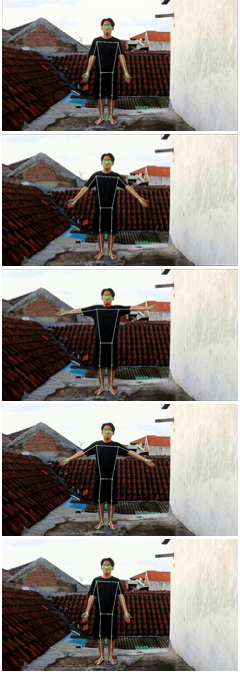
\includegraphics[width=0.33\textwidth]{bab4/ar_Key1.png}}
	\subfloat[]{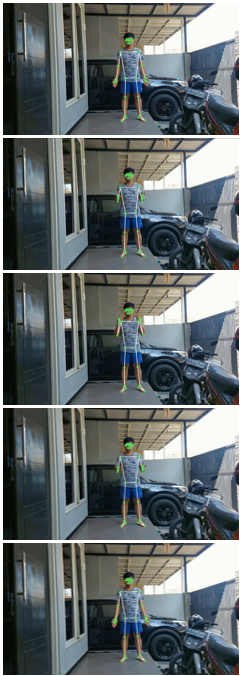
\includegraphics[width=0.33\textwidth]{bab4/ar_Key2.png}}
	\subfloat[]{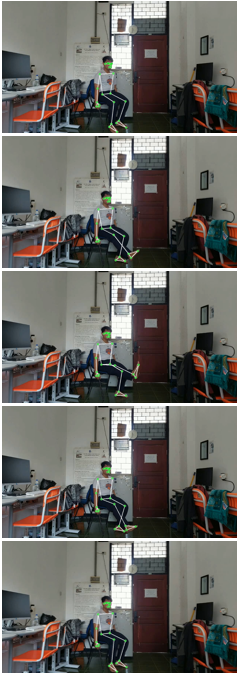
\includegraphics[width=0.33\textwidth]{bab4/ar_Key3.png}}
	\caption{Examples of pose estimation results using mediapipe for exercise activity types (a) adduction abduction, (b) elbow flexion extension, and (c) right knee flexion extension.}
	\label{fig:KeypointViz}
\end{figure}

Each extracted frame provides comprehensive information on the type of exercise activity performed by the subject. By sequentially extracting keypoints for each frame, we were able to build a detailed and dynamic dataset that reflects the entire range of motion in the activity. From this dataset, we were able to see how the position and orientation of the body changed over time, providing deep insight into the biomechanical characteristics of each exercise activity.
% Setiap frame yang diekstrak menyajikan informasi yang lengkap mengenai jenis aktivitas latihan yang dilakukan oleh subjek. Dengan mengekstrak keypoint untuk setiap frame secara berurutan, kami mampu membangun dataset yang mendetail dan dinamis, yang merefleksikan seluruh rangkaian gerakan dalam aktivitas tersebut. Dari dataset ini, kami dapat melihat bagaimana posisi dan orientasi tubuh berubah sepanjang waktu, memberikan wawasan mendalam tentang karakteristik biomekanik dari masing-masing aktivitas latihan.

From the keypoint extraction process, we generate a data array that describes the keypoint position in three dimensions (\(x,y,z)\) and the confidence score. This array shows the (\(x)\), (\(y)\) and (\(z)\) positions for each keypoint with their associated confidence scores, where these scores indicate the accuracy of keypoint detection by the model. The use of three-dimensional data allows us to perform a more detailed analysis of the motion performed, including the depth of motion that cannot be achieved with only two-dimensional data.
% Dari proses ekstraksi keypoint, kami menghasilkan array data yang menggambarkan posisi keypoint dalam tiga dimensi (\(x,y,z)\) dan skor kepercayaan. Array ini menunjukkan posisi (\(x)\), (\(y)\) dan (\(z)\) untuk setiap keypoint dengan skor kepercayaan yang terkait, di mana skor ini mengindikasikan keakuratan deteksi keypoint oleh model. Penggunaan data tiga dimensi memungkinkan kami untuk melakukan analisis yang lebih detil terhadap gerakan yang dilakukan, termasuk kedalaman gerakan yang tidak dapat dicapai hanya dengan data dua dimensi.

\section{Data Training Preparation}
\label{sec:DataTrainingPreparation}
\begin{figure}[]
	\centering
	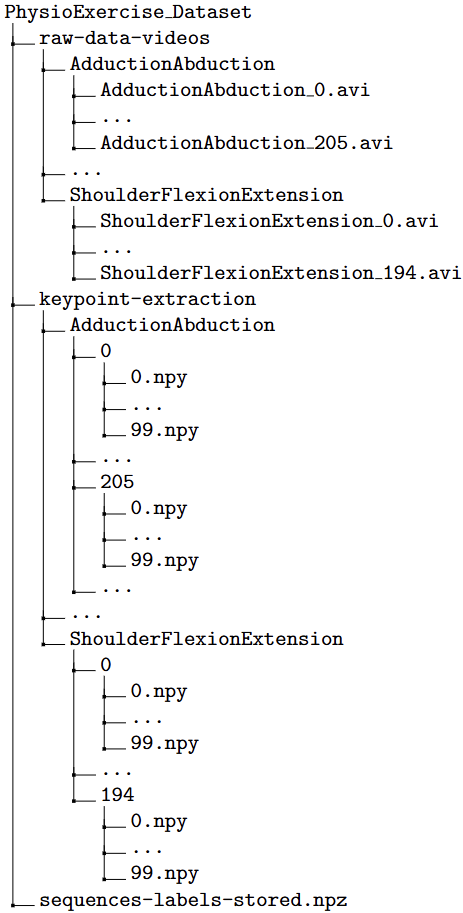
\includegraphics[width=0.7\textwidth]{bab4/ar_DataStructure.png}
	\caption{Data structure of PhysioExercise dataset.}
	\label{fig:DataStructure}
\end{figure}

This section describes the data structure of the dataset that will be used for the training process. The PhysioExercise dataset consists of raw data and data extracted from keypoints using the Mediapipe framework. Figure \ref{fig:DataStructure} shows the data structure of the dataset. The data used in this training is a collection of arrays containing information from images. To get a collection of arrays, the process goes through several stages. The first stage is to collect all video data into a folder. These video data are the raw data that will be extracted from the video frames and keypoints. The amount of data in each class is different, as shown in table \ref{tab:class-dataset}.
% Bagian ini menjelaskan struktur data dari dataset yang akan digunakan untuk proses pelatihan. Dataset PhysioExercise terdiri dari data mentah dan data hasil ekstraksi keypoint menggunakan framework Mediapipe. Gambar \ref{fig:DataStructure} menunjukkan struktur data dari dataset. Data yang digunakan dalam pelatihan ini adalah kumpulan data array yang berisikan informasi dari citra. Untuk mendapatkan kumpulan array, proses dilalui dalam beberapa tahapan. Tahapan pertama adalah mengumpulkan seluruh data video ke dalam sebuah folder. Data-data video ini merupakan data mentah yang akan diekstrak frame video dan keypoint-nya. Jumlah dari data pada setiap kelasnya berbeda-beda, seperti yang ditunjukkan pada tabel \ref{tab:class-dataset}. 

\begin{figure}[h!]
	\centering
	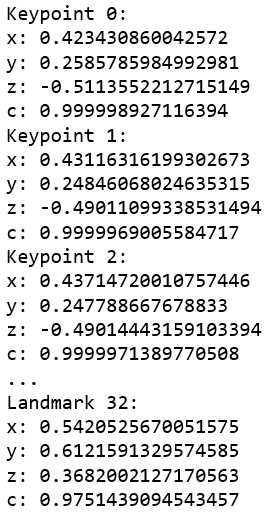
\includegraphics[width=0.33\textwidth]{bab4/ar_KeypointExtractionSample.png}
	\caption{Example of keypoint extraction results for a frame.}
	\label{fig:KeypointExtractionSample}
\end{figure}

After being separated into folders according to class, the data was then extracted for video frames and keypoints. Each data is either extracted into 100 frames which are then pose estimated using the Mediapipe framework. The pose estimation takes the coordinates and visibility of each detected keypoint, following the equation \ref{eq: pers.4}. Figure \ref{fig:KeypointExtractionSample} is an example of keypoint extraction results on a frame. This coordinate data belongs to all frames and is combined for each window into one complete data information. The keypoint extraction results of each frame are stored in '.npy' files so that a video data will have 100 '.npy' files that sequentially carry the exercise activity information.
% Setelah dipisahkan ke dalam folder-folder sesuai dengan kelasnya, data ini kemudian diekstrak frame video dan keypoint-nya. Setiap data entah diekstrak menjadi 100 frame yang kemudian diestmasi pose-nya menggunakan framework Mediapipe. Estimasi pose mengambil koordinat dan visibilitas dari setiap keypoint yang terdeteksi, mengikuti persamaan \ref{eq: pers.4}. Gambar \ref{fig:KeypointExtractionSample} merupakan contoh hasil ekstraksi keypoint pada sebuah frame. Data koordinaat ini dimiliki oleh semua frame dan digabungkan untuk setiap window-nya menjadi satu informasi data yang utuh. Hasil ekstraksi keypoint setiap frame disimpan dalam file '.npy' sehingga sebuah data video akan memiliki 100 file '.npy' yang secara urut membawa informasi akifitas latihan.

\begin{figure}[h!]
	\centering
	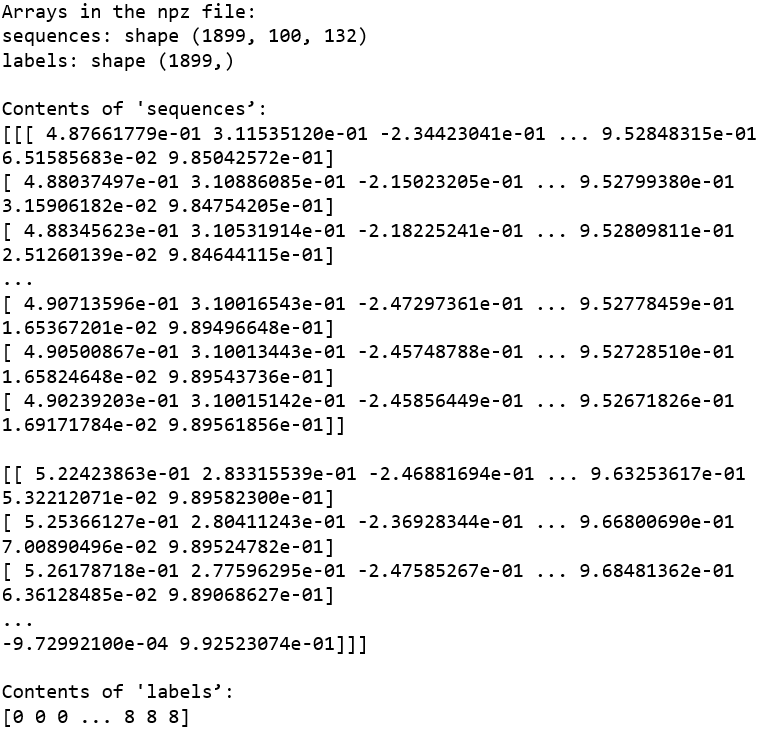
\includegraphics[width=0.8\textwidth]{bab4/ar_npzFile.png}
	\caption{The contents of the '.npz' file that stores sequences and labels data.}
	\label{fig:npzFile}
\end{figure}

To perform training, each extracted data frame is saved into a single file. Each frame generates a set of keypoints that are stored in an array. Frames from one video are collected in one time window to create a sequence. Each window is labeled according to the training activity class. The data is organized following the form of equations \ref{eq: pers.5} and \ref{eq: pers.6}. This array of data is stored in '.npz' format, a format capable of storing multiple arrays. Figure \ref{fig:npzFile} shows the contents of the '.npz' file containing the data ready for the training process.
% Untuk melakukan pelatihan, masing-masing data ekstraksi yang dimiliki kemudian disimpan ke dalam satu file. Setiap frame menghasilkan satu set keypoint yang disimpan dalam array. Frame dai satu video dikumpulkan dalam satu jendela waktu untuk membuat sequence. Masing-masing jendela diberi label sesuai dengan kelas aktifitas latihan. Data yang disusun mengikuti bentuk persamaan \ref{eq: pers.5} dan \ref{eq: pers.6}. Susunan data ini disimpan daa format '.npz', sebuah format yang mampu menyimpan multi array. Gambar \ref{fig:npzFile} menunjukkan isi dari file '.npz' yang berisikan data yang siap untuk prose pelatihan. 



\section{Performance Metrics Evaluation}
\label{sec4:evaluation}

We have trained various deep learning architectures on the PhysioExercise dataset. The tested architectures include CNN, LSTM, CNN-LSTM, and deep CNN-LSTM. From each of these architectures, we managed to develop one best model, which we then compared against each other to evaluate their performance.
% Kami telah melatih berbagai arsitektur deep learning pada dataset PhysioExercise. Arsitektur yang diuji termasuk CNN, LSTM, CNN-LSTM, dan deep CNN-LSTM. Dari setiap arsitektur ini, kami berhasil mengembangkan satu model terbaik, yang kemudian kami bandingkan satu sama lain untuk mengevaluasi kinerja mereka.

\subsection{CNN Model Performance}
\label{subsec4:CNNPerformance}

One of the architectures used in this work is the CNN architecture. This section describes the performance of the CNN model using the PhysioExercise dataset. Figure \ref{fig:CNN_AccLoss} is the accuracy and loss graph for training and validation data. This graph provides an overview of how the model behaves during the training and validation process using the CNN architecture. The training was done in 100 epochs. In the initial 20 epochs, the model experienced a fairly high increase in accuracy. The increase occurred around 0.2 to 0.6 in these first 20 epochs. After entering the 21st epoch, the training accuracy continued to increase and stabilized at around 0.8 accuracy, while the validation accuracy fluctuated between 0.7 to 0.8. This fluctuation shows that the model experienced some overfitting at some points. This overfitting indicates that the model is too adaptive to the training data and less able to generalize to the validation data.
% Salah satu arsitektur yang digunakan pada pekerjaan ini adalah arsitektur CNN. Bagian ini menjelaskan peforma dari model CNN menggunakan dataset PhysioExercise. Gambar \ref{fig:CNN_AccLoss} adalah grafik akurasi dan loss untuk data latih dan validasi. Grafik ini memberikan gambaran umum bagaimana model berperilaku selama proses pelatihan dan validasi menggunakan arsitektur CNN. Pelatihan dilakukan dalam 100 epoch. Pada 20 epoch awal, model mengalami peningkatan akurasi yang cukup tinggi. Peningkatan terjadi sekitar 0.2 menjadi 0.6 dalam 20 epoch pertama ini. Setelah memasuki epoch ke 21, akurasi pelatihan terus meningkat dan stabil pada kisaran akurasi 0.8, sedangkan akurasi validasi mengalami fluktuasi antara 0.7 hingga 0.8. Fluktuasi ini menunjukkan model mengalami beebrapa overfitting pada beberapa titik. Overfitting ini menunjukkan model terlalu menyesuaikan dengan data latih dan kurang dapat generalisasi ke data validasi.

\begin{figure}[h!]
	\centering
	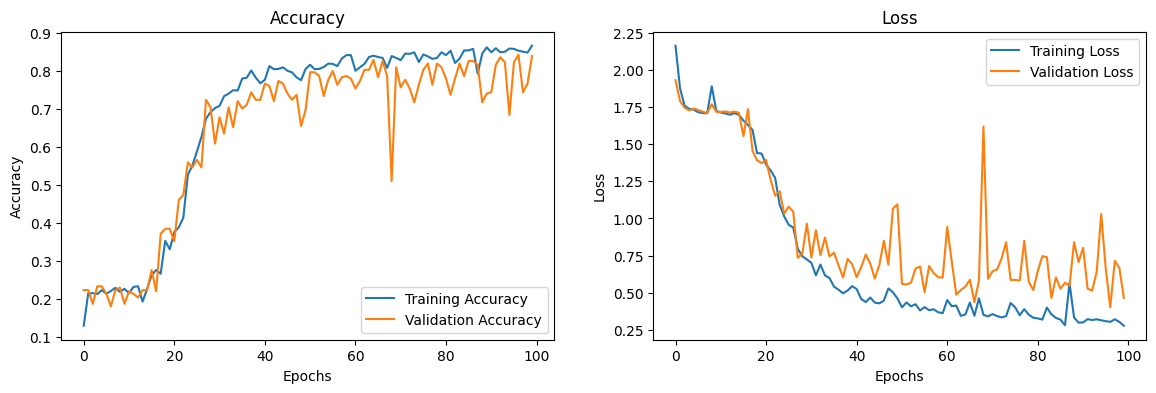
\includegraphics[width=1\textwidth]{bab4/ar_CNN_AccLoss.png}
	\caption{Accuracy and loss of training and validation on the CNN model.}
	\label{fig:CNN_AccLoss}
\end{figure}

In the first 20 epochs of the loss graph, the model loss has decreased dramatically to below 1.0. This value shows that the model is starting to be able to predict accurately. Training and validation loss tend to decrease until the end of training. However, validation loss does not decrease as well as training loss. In addition, the validation loss experiences several peaks and significant fluctuations. This graph once again shows an overfitting model and a lack of generalization to the validation data.
% Pada 20 epoch pertama dari grafik kehilangan, kehilangan model telah menurun secara dramatis hingga di bawah 1,0. Nilai ini menunjukkan model mulai mampu melakukan prediksi dengan akurat. Training dan validation loss cenderung menurun hingga akhir pelatihan. Namun, validation loss tidak menurun sebaik training loss. Selain itu, loss validasi mengalami beberapa kali puncakd an fluktuasi yang signifikan. Grafik ini sekali lagi menunjukkan model yang overfitting dan kurang mampu generalisasi ke data validasi.

\begin{figure}[h!]
	\centering
	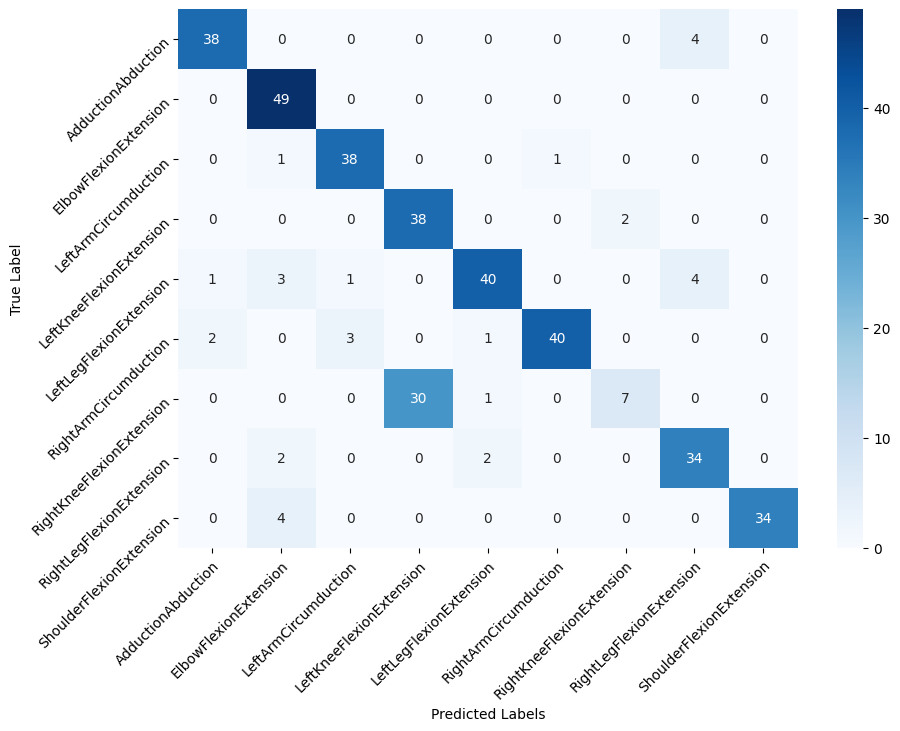
\includegraphics[width=1\textwidth]{bab4/ar_CNN_Confmatrix.png}
	\caption{Confusion matrix of the CNN model outcomes.}
	\label{fig:CNN_Confmatrix}
\end{figure}

The confusion matrix shown in figure \ref{fig:CNN_Confmatrix} provides a visual representation of the performance of the CNN model in classifying exercise activities for the elderly. Each row of the confusion matrix shows the actual number of instances for each class, while each column shows the number of instances predicted by the model for each class. There are 4 classes that show excellent performance, namely in the ElbowFlexionExtension, LeftArmCircumduction, RightArmCircumduction, and ShoulderFlexionExtension classes. The model predictions in these classes closely match the actual labels, with 49, 38, 30, and 34 correctly classified instances, respectively.
% Confusion matrix yang ditampilkan pada gambar \ref{fig:CNN_Confmatrix} memberikan gambaran visual tentang performa model CNN dalam mengklasifikasikan aktivitas latihan untuk elderly. Setiap baris dari confusion matrix menunjukkan jumlah instance aktual untuk setiap kelas, sementara setiap kolom menunjukkan jumlah instance yang diprediksi oleh model untuk setiap kelas. Terdapat 4 kelas yang menunjukkan peforma sangat baik, yaitu pada kelas ElbowFlexionExtension, LeftArmCircumduction, RightArmCircumduction, dan ShoulderFlexionExtension. Prediksi model pada kelas ini sangat sesuai dengan label sebenarnya, dengan masing-masing memiliki 49, 38, 30, dan 34 instance yang diklasifikasikan dengan benar. 

However, there are classes that experience significant confusion in making predictions. That class is RightKneeFlexionExtension. Of the 38 instances in the RightKneeFlexionExtension class, only 7 were correctly classified, while 30 instances were classified as LeftKneeFlexionExtension. These errors contributed to the low precision and recall of these classes, as shown in the classification report. This misclassification can occur based on several factors. One of the main factors is the similarity in motion between the two. The model failed to predict the RightKneeFlexionExtension instance instead classifying it as LeftKneeFlexionExtension. The similar features between the two are the main reason for the model's confusion in classifying correctly. Although the model showed good ability in classifying most of the classes, further improvement is needed to reduce confusion between classes that have movements that may be visually similar.
% Akan tetapi, terdapat kelas yang mengalami kebingungan signifikan dalam melakukan prediksi. Kelas tersebut adalah RightKneeFlexionExtension. Dari 38 instance pada kelas RightKneeFlexionExtension, hanya 7 yang diklasifikasikan dengan benar, sementara 30 instance diklasifikasikan sebagai LeftKneeFlexionExtension. Kesalahan ini berkontribusi pada rendahnya precision dan recall pada kelas-kelas tersebut, seperti yang ditunjukkan pada classification report. Kesalahan dalam klasifikasi ini dapat terjadi berdasarkan beberap faktor. Salah satu faktor utamanya adalah kemiripan gerakan diantara keduanya. Model gagal memprediksi instance RightKneeFlexionExtension alih-alih mengklasifikasikannya sebagai LeftKneeFlexionExtension. Fitur yang mirip diantara keduanya menjadi alasan utama model mengalami kebingungan dalam mengklasifikasikan dengan benar. Meskipun model menunjukkan kemampuan yang baik dalam mengklasifikasikan sebagian besar kelas, peningkatan lebih lanjut diperlukan untuk mengurangi kebingungan antar kelas yang memiliki gerakan yang mungkin secara visual mirip.

\begin{table}[h!]
	\centering
	\caption{Classification report of the CNN model.}
	\label{tab:CNNreport}
	\begin{tabular}{rrrrr}
		\multicolumn{1}{l}{}      & precision            & recall               & f1-score             & support              \\
		\multicolumn{1}{l}{}      &                      &                      &                      &                      \\
		AdductionAbduction        & 0.93                 & 0.90                 & 0.92                 & 42                   \\
		ElbowFlexionExtension     & 0.83                 & 1.00                 & 0.91                 & 49                   \\
		LeftArmCircumduction      & 0.90                 & 0.95                 & 0.93                 & 40                   \\
		LeftKneeFlexionExtension  & 0.56                 & 0.95                 & 0.70                 & 40                   \\
		LeftLegFlexionExtension   & 0.91                 & 0.82                 & 0.86                 & 49                   \\
		RightArmCircumduction     & 0.98                 & 0.87                 & 0.92                 & 46                   \\
		RightKneeFlexionExtension & 0.78                 & 0.18                 & 0.30                 & 38                   \\
		RightLegFlexionExtension  & 0.81                 & 0.89                 & 0.85                 & 38                   \\
		ShoulderFlexionExtension  & 1.00                 & 0.89                 & 0.94                 & 38                   \\
		\multicolumn{1}{l}{}      & \multicolumn{1}{l}{} & \multicolumn{1}{l}{} & \multicolumn{1}{l}{} & \multicolumn{1}{l}{} \\
		accuracy                  &                      &                      & 0.84                 & 380                  \\
		macro avg                 & 0.85                 & 0.83                 & 0.81                 & 380                  \\
		weighted avg              & 0.86                 & 0.84                 & 0.82                 & 380
	\end{tabular}%
\end{table}

Table \ref{tab:CNNreport} presents the classification report for the model using CNN architecture. Evaluation using the classification report shows the precision, recall, and f1-score metrics for each activity. This classification model has shown quite good performance. Overall, the accuracy of this model is 84\%. The overall results for each metric were calculated using macro averaging and weighted averaging methods. Using macro averaging, the average results for precision, recall, and f1-score of this model are 0.85, 0.83, and 0.81 respectively. Unlike the macro averaging method, calculations using the weighted averaging method showed a precision of 0.86, recall of 0.84, and F1-score of 0.82. This method is more representative of the class distribution in a dataset.
% Tabel \ref{tab:CNNreport} menyajikan classification report untuk model menggunakan CNN arsitektur. Evaluasi menggunakan classification report menunjukkan metris precision, recall, dan F1-score untuk setiap aktifitas. Model klasifikasi ini telah menunjukkan peforma yang cukup baik. Secara keseluruhan, akurasi model ini sebesar 84\%. Hasil keseluruhan pada setiap metrisnya dihitung menggunakan metode macro averaging dan weighted averaging. Menggunakan macro averaging, hasil rata-rata untuk precision, recall, dan F1-score model ini sebesar 0.85, 0.83, dan 0.81 respectively. Berbeda dengan metode macro averaging, perhitungan menggunakan metode weighted averaging menunjukkan hasil precision sebesar 0.86, recall sebesar 0.84, dan F1-score sebesar 0.82. Metode ini lebih representatif terhadap distribusi kelas dalam sebuah dataset.

The ShoulderFlexionExtension and RightArmCircumduction classes have very high precision, reaching 1.00 and 0.98 respectively. This value indicates that there are very few false positives in the predictions for these activities. This explanation is in line with the confusion matrix results where these classes can predict all instances well. However, the model showed difficulty with the RightKneeFlexionExtension class with a precision of only 0.78 and recall of 0.18. This indicates a large number of false negatives that affect the model's ability to detect this activity. The LeftKneeFlexionExtension activity also has a relatively low precision of 0.56 although the recall is quite high at 0.95, indicating that the model often incorrectly predicts this class as another activity.
% Kelas ShoulderFlexionExtension dan RightArmCircumduction memiliki precision yang sangat tinggi, masing-masing mencapai 1.00 dan 0.98. Nilai ini menunjukkan sedikitnya false positives pada prediksi untuk aktifitas ini. Penjelasan ini selaras dengan hasil confusion matrix di mana kelas ini dapat memprediksi seluruh instance dengan baik. Namun, model menunjukkan kesulitan pada kelas RightKneeFlexionExtension dengan precision hanya 0.78 dan recall 0.18. Nilai ini mengindikasikan banyaknya false negatives yang mempengaruhi kemampuan model dalam mendeteksi aktifitas ini. Aktifitas LeftKneeFlexionExtension juga memiliki precision yang relatif rendah sebesar 0.56 meskipun recall cukup tinggi pada 0.95, menunjukkan bahwa model sering salah dalam memprediksi kelas ini sebagai aktifitas lain.

\begin{table}[h!]
	\caption{Accuracy results for training, validation, and test data of the CNN model.}
	\label{tab:CNNAccuracy}
	\centering
	\begin{tabular}{|c|c|c|}
		\hline
		Training accuracy (\%) & Validation accuracy (\%) & Test accuracy (\%) \\ \hline
		86.83                  & 83.83                    & 83.68              \\ \hline
	\end{tabular}
\end{table}

Table \ref{tab:CNNAccuracy} is a summary of the accuracy for training, validation, and test data. Of the three, the accuracy value of the CNN model shows a consistent value. The model achieved a training accuracy of 86.83\%, which shows that the model is able to learn well from the training data. The validation accuracy of 83.83\% shows that the model has a good generalization ability to data not seen during training. Both accuracy results are consistent with the previous accuracy-loss graph where the validation accuracy remains stable around 0.83 after 20 epochs. The test accuracy value of 83.68\% confirms that the model performance remains stable when tested on an entirely new dataset. This indicates that the model did not experience significant overfitting. This is also supported by the classification report and confusion matrix which show that most classes are well classified, although there are some classes that show lower performance such as RightKneeFlexionExtension. The consistency between training, validation and test accuracies shows that the model performs reliably in this classification task, although there is still room for improvement especially in classes that show higher misclassification.
% Tabel \ref{tab:CNNAccuracy} merupakan rangkuman dari akurasi untuk data training, validasi, dan test. Dari ketiganya, nilai akurasi model CNN menunjukkan nilai yang konsisten. Model mencapai akurasi pelatihan sebesar 86.83\%, yang menunjukkan bahwa model mampu belajar dengan baik dari data pelatihan. Akurasi validasi sebesar 83.83\% menunjukkan bahwa model memiliki kemampuan generalisasi yang baik terhadap data yang tidak terlihat selama pelatihan. Kedua hasil akurasi ini konsisten dengan grafik akurasi-loss sebelumnya di mana akurasi validasi tetap stabil di sekitar 0.83 setelah 20 epoch. Nilai akurasi uji sebesar 83.68\% mengkonfirmasi bahwa performa model tetap stabil ketika diuji pada dataset yang sepenuhnya baru. Kondisi ini mengindikasikan bahwa model tidak mengalami overfitting yang signifikan. Hal ini juga didukung oleh classification report dan confusion matrix yang menunjukkan bahwa sebagian besar kelas diklasifikasikan dengan baik, meskipun terdapat beberapa kelas yang menunjukkan performa lebih rendah seperti RightKneeFlexionExtension. Konsistensi antara akurasi pelatihan, validasi, dan uji menunjukkan bahwa model memiliki performa yang andal dalam tugas klasifikasi ini, meskipun masih ada ruang untuk perbaikan terutama pada kelas-kelas yang menunjukkan kesalahan klasifikasi yang lebih tinggi.

\subsection{LSTM Model Performance}
\label{subsec4:LSTMPerformance}

\begin{figure}[h!]
	\centering
	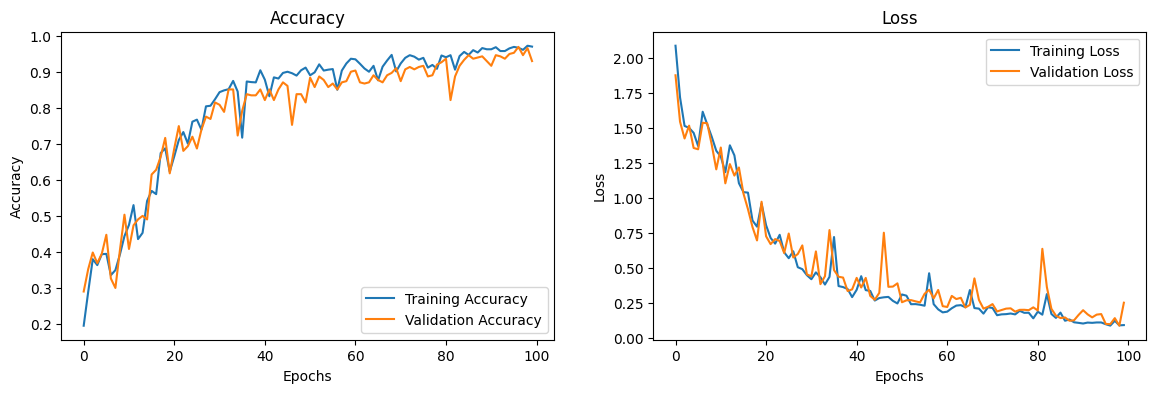
\includegraphics[width=1\textwidth]{bab4/ar_LSTM_AccLoss.png}
	\caption{Accuracy and loss of training and validation on the LSTM model.}
	\label{fig:LSTM_AccLoss}
\end{figure}

Training of the PhysioExercise dataset was also performed using the LSTM architecture. Figure \ref{fig:LSTM_AccLoss} represents the accuracy and loss graphs for training and validation data for each training epoch. The training has been done in 100 epochs. The accuracy graph on the left depicts the increase in accuracy in both the training data (Training Accuracy) and validation data (Validation Accuracy). At the beginning of training, both accuracies increase rapidly, indicating that the model immediately starts learning patterns from the data. Validation accuracy also shows an increasing trend, although there are some larger fluctuations. These fluctuations indicate a slight overfitting but overall it still generalizes well to the untrained data.
% Pelatihan dataset PhysioExercise juga dilakukan menggunakan arsitektur LSTM. Gambar \ref{fig:LSTM_AccLoss} merupakan grafik akurasi dan loss untuk data training dan validasi setiap epoch pelatihan. Pelatihan telah dilakukan dalam 100 epoch. Grafik akurasi di sebelah kiri menggambarkan peningkatan akurasi baik pada data pelatihan (Training Accuracy) maupun data validasi (Validation Accuracy). Pada awal pelatihan, kedua akurasi meningkat dengan cepat, mengindikasikan bahwa model segera mulai belajar pola dari data. Akurasi validasi juga menunjukkan tren peningkatan, meskipun terdapat beberapa fluktuasi yang lebih besar. Fluktuasi ini mengindikasikan adanya sedikit overfitting namun secara keseluruhan tetap mampu generalisasi dengan baik ke data yang tidak dilatih.

The loss graph on the right illustrates the decrease in loss in both the training data (Training Loss) and the validation data (Validation Loss). At the beginning of training, both losses decrease rapidly. The rapidly decreasing loss values indicate that the model is quickly reducing the prediction error. The training loss continues to decrease and approaches zero, indicating that the model is almost perfect on the training data. Meanwhile, the validation loss also decreases but with larger fluctuations, indicating that there are some epochs where the model does not predict the validation data as accurately as in other epochs. This fluctuation could be an indication of overfitting, where the model learns too specifically on the training data and is less able to generalize to new data. On the other hand, the validation loss value is still above the training loss value by quite a distance.
% Grafik loss di sebelah kanan menggambarkan penurunan loss baik pada data pelatihan (Training Loss) maupun data validasi (Validation Loss). Pada awal pelatihan, kedua loss menurun dengan cepat. Nilai loss yang menurun dengan cepat menunjukkan bahwa model dengan cepat mengurangi kesalahan prediksi. Loss pelatihan terus menurun dan mendekati nol, mengindikasikan bahwa model hampir sempurna pada data pelatihan. Sementara itu, loss validasi juga menurun tetapi dengan fluktuasi yang lebih besar, menunjukkan adanya beberapa epoch di mana model tidak memprediksi data validasi seakurat pada epoch lainnya. Fluktuasi ini dapat menjadi indikasi overfitting, di mana model belajar terlalu spesifik pada data pelatihan dan kurang mampu generalisasi pada data baru. Di sisi lain, nilai loss validasi masih berada di atas dari nilai loss training cukup jauh.

\begin{figure}[h!]
	\centering
	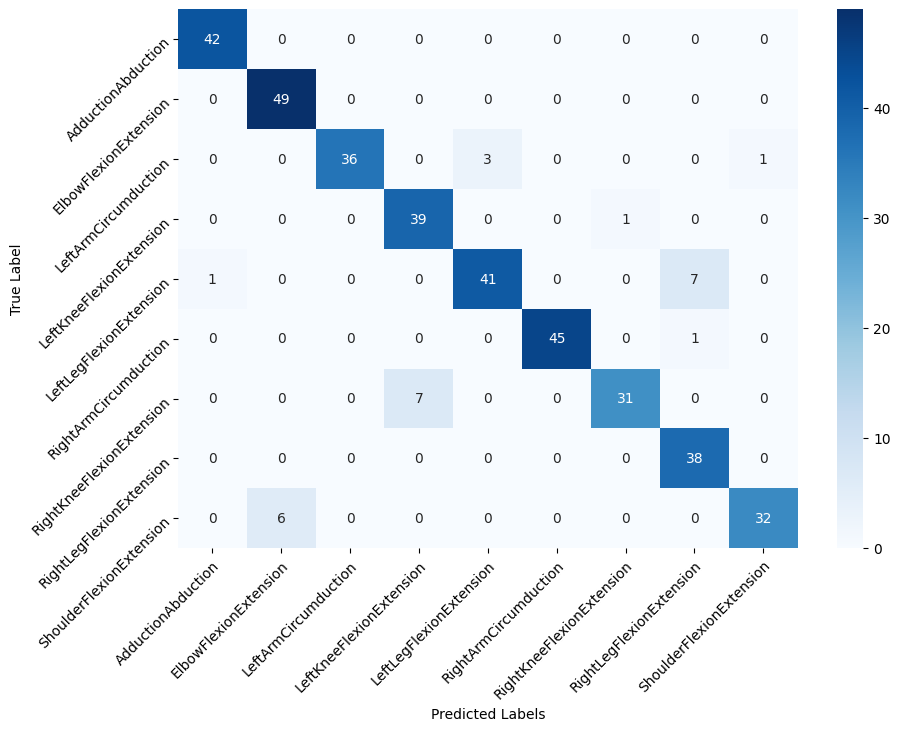
\includegraphics[width=1\textwidth]{bab4/ar_LSTM_Confmatrix.png}
	\caption{Confusion matrix of the LSTM model outcomes.}
	\label{fig:LSTM_Confmatrix}
\end{figure}

The confusion matrix of the LSTM model for classification of exercise activities in the elderly is shown in figure \ref{fig:LSTM_Confmatrix}. This confusion matrix describes the number of correct predictions (main diagonal) and misclassifications (off-diagonal) for each class. Looking at the main diagonal, it appears that the model managed to classify most of the data correctly. Some examples are in the AdductionAbduction activity with 42 correctly classified data, ElbowFlexionExtension with 49 correctly classified data, and RightLegFlexionExtension with 38 correctly classified data. However, there are some classes that experience errors in classification. For example, the LeftLegFlexionExtension class predicts 7 data as RightLegFlexionExtension, and the RightKneeFlexionExtension class predicts 6 data as LeftKneeFlexionExtension.
% Confusion matrix model LSTM untuk klasifikasi aktivitas latihan pada elderly, ditunjukkan pada gambar \ref{fig:LSTM_Confmatrix}. Confusion matrix ini menjelaskan jumlah prediksi yang benar (diagonal utama) dan kesalahan klasifikasi (off-diagonal) untuk setiap kelasnya. Melihat diagonal utama, tampak bahwa model berhasil mengklasifikasikan sebagian besar data dengan benar. Beberapa contohnya adalah pada aktifitas AdductionAbduction dengan 42 data terklasifikasi dengan benar, ElbowFlexionExtension dengan 49 data terklasifikasi dengan benar, dan RightLegFlexionExtension dengan 38 data terklasifikasi dengan benar. Akan tetapi, terdapat beberapa kelas yang mengalami kesalahan dalam klasifikasi. Sebagai contoh, kelas LeftLegFlexionExtension memprediksi 7 data sebagai RightLegFlexionExtension, dan pada kelas RightKneeFlexionExtension memprediksi 6 data sebagai LeftKneeFlexionExtension.

As a further analysis, misclassification often occurs in classes that have similar or adjacent activities in the motion space, such as LeftLegFlexionExtension and RightLegFlexionExtension. However, the model as a whole performed quite well with high accuracy in the majority of the classes, especially AdductionAbduction, ElbowFlexionExtension, and RightLegFlexionExtension. The misclassifications indicate that although the LSTM model is solid, there is room for further improvement, such as by adding more training data or tweaking the model to improve the classification ability on hard-to-distinguish classes. Thus, this confusion matrix provides deeper insight into the model's performance in classifying exercise activities in the elderly, supports the previously described analysis, and shows areas where the model can still be improved.
% Sebagai analisis lebih lanjut, kesalahan klasifikasi sering terjadi pada kelas-kelas yang memiliki aktifitas mirip atau berdekatan dalam ruang geraknya, seperti pada LeftLegFlexionExtension dan RightLegFlexionExtension. Meskipun demikian, model secara keseluruhan memiliki peforma cukup baik dengan tingkat akurasi tinggi pada mayoritas kelas, khususnya AdductionAbduction, ElbowFlexionExtension, dan RightLegFlexionExtension. Kesalahan klasifikasi yang terjadi mengindikasikan bahwa meskipun model LSTM ini solid, ada ruang untuk perbaikan lebih lanjut, seperti dengan menambah lebih banyak data pelatihan atau melakukan penyesuaian model untuk meningkatkan kemampuan klasifikasi pada kelas-kelas yang sulit dibedakan. Dengan demikian, confusion matrix ini memberikan wawasan yang lebih dalam tentang performa model dalam mengklasifikasikan aktivitas latihan pada elderly, mendukung analisis yang telah dijelaskan sebelumnya, dan menunjukkan area-area di mana model masih dapat diperbaiki.

\begin{table}[h!]
	\centering
	\caption{Classification report of the LSTM model.}
	\label{tab:LSTMreport}
	\begin{tabular}{rrrrr}
		\multicolumn{1}{l}{}      & precision            & recall               & f1-score             & support              \\
		\multicolumn{1}{l}{}      &                      &                      &                      &                      \\
		AdductionAbduction        & 0.98                 & 1.00                 & 0.99                 & 42                   \\
		ElbowFlexionExtension     & 0.89                 & 1.00                 & 0.94                 & 49                   \\
		LeftArmCircumduction      & 1.00                 & 0.90                 & 0.95                 & 40                   \\
		LeftKneeFlexionExtension  & 0.85                 & 0.97                 & 0.91                 & 40                   \\
		LeftLegFlexionExtension   & 0.93                 & 0.84                 & 0.88                 & 49                   \\
		RightArmCircumduction     & 1.00                 & 0.98                 & 0.99                 & 46                   \\
		RightKneeFlexionExtension & 0.97                 & 0.82                 & 0.89                 & 38                   \\
		RightLegFlexionExtension  & 0.83                 & 1.00                 & 0.90                 & 38                   \\
		ShoulderFlexionExtension  & 0.97                 & 0.84                 & 0.90                 & 38                   \\
		\multicolumn{1}{l}{}      & \multicolumn{1}{l}{} & \multicolumn{1}{l}{} & \multicolumn{1}{l}{} & \multicolumn{1}{l}{} \\
		accuracy                  &                      &                      & 0.93                 & 380                  \\
		macro avg                 & 0.93                 & 0.93                 & 0.93                 & 380                  \\
		weighted avg              & 0.94                 & 0.93                 & 0.93                 & 380
	\end{tabular}%
\end{table}

An explanation of the classification report of the LSTM model is shown in table \ref{tab:LSTMreport}. This table reports the precision, recall, f1-score, and support metrics for each class, as well as macro averaging and weighted averaging of the entire model. The precision value measures the correct positive predictions out of all positive predictions made by the model. A higher precision indicates the model makes fewer errors in predicting a particular class. Based on the table \ref{tab:LSTMreport}, LeftArmCircumduction and RightArmCircumduction have a precision value of 1.00. This result shows that the model is able to predict this class well, even though they are both activities with adjacent motion spaces. RightLegFlexionExtension is the class with the lowest precision among the other classes with a precision value of 0.83. Even so, this value is still considered high for prediction work. On the other hand, recall is a metric that measures the proportion of actual instances of a class that are correctly identified by the model. In this LSTM model, there are three classes with perfect recall values, i.e., AdductionAbduction, ElbowFlexionExtension, and RightLegFlexionExtension. This value indicates that the model is able to predict these classes perfectly. The lowest recall value in this LSTM model is in the RightKneeFlexionExtension class with a value of 0.82. This value is still relatively high even though the error rate is the highest compared to other classes.
% Penjelasan mengenai classification report model LSTM ditunjukkan pada tabel \ref{tab:LSTMreport}. Tabel ini menyajikan laporan metrik precision, recall, f1-score, dan support untuk setiap kelas, serta macro averaging dan weighted averaging keseluruhan model. Nilai precision mengukur prediksi positif yang benar dari keseluruhan prediksi positif yang dibuat oleh model. Precision yang semakin tinggi menunjukkan model membuat sedikit kesalahan dalam memprediksi kelas tertentu. Berdasarkan tabel \ref{tab:LSTMreport}, LeftArmCircumduction dan RightArmCircumduction memiliki nilai precision 1.00. Hasil ini menunjukkan model mampu memprediksi kelas ini dengan baik, meskipun keduanya merupakan aktifitas dengan ruang gerak berdekatan. RightLegFlexionExtension menjadi kelas dengan tingkat precision paling rendah di antara kelas-kelas lainnya dengan nilai precision sebesar 0.83. Meski begitu, nilai ini masih dianggap tinggi untuk dalam pekerjaan prediksi. Di sisi lain, recall merupakan metrik yang mengukur proporsi instance sebenarnya dari sebuah kelas yang berhasil diidentifikasi dengan benar oleh model. Pada model LSTM ini, terdapat tiga kelas dengan nilai recall sempurna, yaitu AdductionAbduction, ElbowFlexionExtension, dan RightLegFlexionExtension. Nilai ini menunjukkan model mampu memprediksi dengan sempurna atas kelas-kelas tersebut. Nilai recall terendah pada model LSTM ini berada pada kelas RightKneeFlexionExtension dengan nilai 0.82. Nilai ini masih tergolong tinggi meskipun tingkat kekeliruannya paling banyak dibandingkan dengan kelas lainnya.

F1-score gives the average harmony of precision and recall which shows the balance between these two metrics. The classes with the highest f1-score values are AdductionAbduction and RightArmCircumduction with f1-score values of 0.99. The lowest value for this metric is 0.88 for the LeftLegFlexionExtension class. This value corresponds to its lowest recall value compared to the recall of other classes. These metrics are overall modeled using macro averaging and weighted averaging methods. In the macro averaging method, the precision, recall, and f1-score metrics have the same value, which is 0.93. On the other hand, the values of the three using the weigthed averaging method have values of 0.94, 0.93, and 0.93 respectively. Weighted averaging is considered more representative of the class distribution in a dataset.
% F1-score memberikan rata-rata keharmonisan precision dan recall dimana menunjukkan keseimbangan di antara kedua metric ini. Kelas-kelas dengan nilai f1-score tertinggi berada pada kelas AdductionAbduction dan RightArmCircumduction dengan nilai f1-score sebesar 0.99. Nilai terendaha pada metric ini adalah 0.88 pada kelas LeftLegFlexionExtension. Nilai ini berhubungan dengan nilai recall-nya yang paling rendah dibandingkan dengan recall kelas lainnya. Metric-metric ini secara keseluruhan model ditunjukkan menggunakan metode macro averaging dan weighted averaging. Pada metode macro averaging, metric precision, recall, dan f1-score memiliki nilai yang sama, yaitu 0.93. Di sisi lain, nilai ketiganya menggunakan metode weigthed averaging memiliki nilai sebesar 0.94, 0.93, dan 0.93 masing-masing. Weighted averaging dianggap lebih representatif terhadap distribusi kelas dalam sebuah dataset.

\begin{table}[h!]
	\caption{Accuracy results for training, validation, and test data of the CNN model.}
	\label{tab:LSTMAccuracy}
	\centering
	\begin{tabular}{|c|c|c|}
		\hline
		Training accuracy (\%) & Validation accuracy (\%) & Test accuracy (\%) \\ \hline
		94.93                  & 93.07                    & 92.89              \\ \hline
	\end{tabular}
\end{table}

We also measured the model accuracy for each training, validation, and test data. Table \ref{tab:LSTMAccuracy} shows the accuracy value of the model for each of these data. The training accuracy reaches 94.93\% which means the model is able to learn the patterns from the training data very well. The validation accuracy reached 93.07\%. Both values are in line with the accuracy-loss graph in figure\ref{fig:LSTM_AccLoss}, where the validation accuracy is not higher than the training accuracy. The ability of the model is shown in the test accuracy, where the data given is data that has never been read by the model. The test accuracy of this model is 92.89\%. This value indicates that the generalization ability of the model is quite good.
% Kami juga mengukur tingkat akurasi model untuk setiap data latih, validasi, dan test. Tabel \ref{tab:LSTMAccuracy} menunjukkan nilai akurasi model setiap data tersebut. Akurasi pelatihan mencapai 94.93\% yang mana model mampu mempelajari pola dari data pelatihan dengan sangat baik. Adapun akurasi validasinya mencapai 93.07\%. Nilai keduanya sejalan dengan grafik akurasi-loss pada gambar\ref{fig:LSTM_AccLoss}, di mana akurasi validasi tidak lebih tinggi dibandingkan dengan akurasi pelatihannya. Kemampuan model ditunjukkan pada akurasi test, di mana data yang diberikan merupakan data yang belum pernah dibaca oleh model. Besar akurasi test model ini adalah 92.89\%. Nilai ini mengindikasikan kemampuan generalisasi model yang cukup baik. 

\subsection{CNN-LSTM Model Performance}
\label{subsec4:CNNLSTMPerformance}

\begin{figure}[h!]
	\centering
	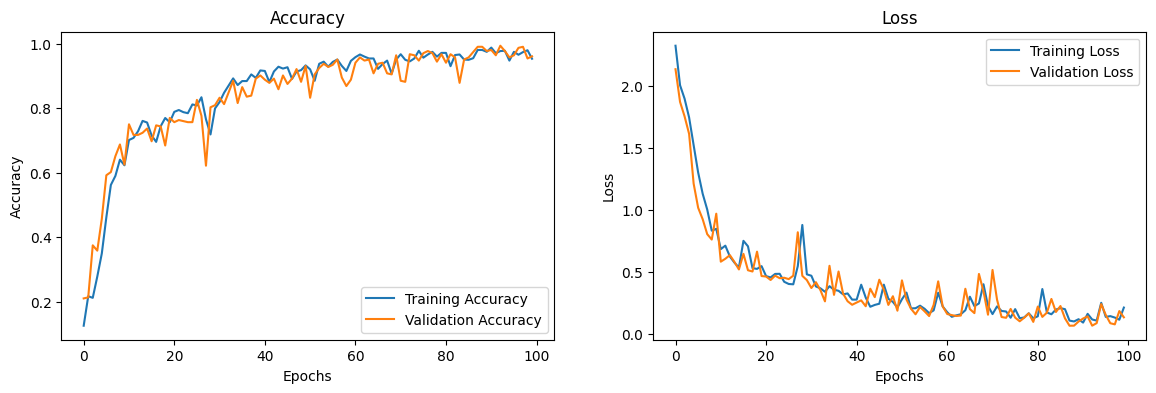
\includegraphics[width=1\textwidth]{bab4/ar_CNNLSTM_AccLoss.png}
	\caption{Accuracy and loss of training and validation on the CNN-LSTM model.}
	\label{fig:CNNLSTM_AccLoss}
\end{figure}

Another architecture used in this work is the CNN-LSTM architecture. Figure \ref{fig:CNNLSTM_AccLoss} provides an overview of the model in learning the PhysioExercise dataset. There are accuracy and loss graphs for training and validation data. The training has been done in 100 epochs. The left graph shows the accuracy of the model for each epoch. A significant improvement occurs in the first 15 epochs for training accuracy. This significant increase indicates that the model is able to learn the data patterns very well. In the following epochs, the training accuracy continues to increase until the end of the training. Although on several occasions the training accuracy had decreased, the trend in training accuracy continued to rise. Similarly, the validation accuracy experienced a significant increase for the first 15 epochs. Then the increase in accuracy occurs until the end of training although the fluctuations that occur are greater than the training accuracy. Fluctuations between training and validation accuracy occurred several times but the trend still showed an increase in accuracy until the training ended.

% Arsitektur lain yang digunakan dalam pekerjaan ini adalah arsitektur CNN-LSTM. Gambar \ref{fig:CNNLSTM_AccLoss} memberikan gambaran umum model dalam mempelajari dataset PhysioExercise. Terdapat grafik akurasi dan loss untuk data pelatihan dan validasi. Pelatihan telah dilakukan dalam 250 epoch. Grafik sebelah kiri menampilkan akurasi model setiap epochnya. Peningkatan yang cukup signifikan terjadi pada 50 epoch pertama untuk akurasi pelatihan. Peningkatan yang signifikan ini menandai model mampu mempelajari pola data dengan sangat baik. Pada epoch berikutnya, akurasi pelatihan terus mengalami kenaikan hingga akhir pelatihan. Meskipun pada beberapa kesempatan akurasi pelatihan sempat mengalami penurunan, namun tren yang terjadi pada akurasi pelatihan tetap naik. Begitu pula pada akurasi validasi, akurasi ini mengalami kenaikan yang signifikan untuk 50 epoch pertama. Kemudian kenaikan akurasi terjadi hingga akhir pelatihan meskipun fluktuasi yang terjadi lebih besar dibandingkan akurasi pelatihannya. Fluktuasi antara akurasi training maupun validasi terjadi beberapa kali namun tren masih menunjukkan kenaikan akurasi hingga pelatihan berakhir.


The loss graph shows the error rate made by the model in learning the data pattern. The loss value decreased significantly in the first 15 epochs. This graph trend applies to both training and validation losses. This decreasing loss trend continues until the end of training although fluctuations in both occur. Similar to accuracy, the loss graph fluctuates throughout the training. This fluctuation shows the ability of the model to learn the given data pattern. The validation graph has larger fluctuations when compared to the training graph. This shows the ability of the model to learn the data several times overfitting. However, the difference between the two values does not show a high number so that the model's ability to generalize data patterns is still considered good.

% Grafik loss menunjukkan tingkat kesalahan yang dilakukan oleh model dalam mempelajari pola data. Nilai loss mengalami penurunan yang cukup signifikan pada 50 epoch pertama meskipun sempat terjadi pelonjakan pada epoch ke 14. Tren grafik ini berlaku untuk loss pelatihan maupun validasi. Tren loss yang menurun ini terus berlangsung hingga akhir pelatihan meskipun fluktuasi pada keduanya terjadi. Sama halnya dengan akurasi, grafik loss ini mengalami fluktuasi disepanjang pelatihan. Fluktuasi ini menunjukkan kemampuan model dalam mempelajari pola data yang diberikan. Grafik validasi memiliki fluktuasi yang lebih besar apabila dibandingkan dengan grafik pelatihan. Hal ini menunjukkan kemampuan model dalam mepelajari data mengalami beberapa kali overfitting. Namun, perbedaan nilai keduanya tidak menunjukkan angka yang tinggi sehingga kemampuan model dalam generalisasi pola data masih dianggap baik.

\begin{figure}[h!]
	\centering
	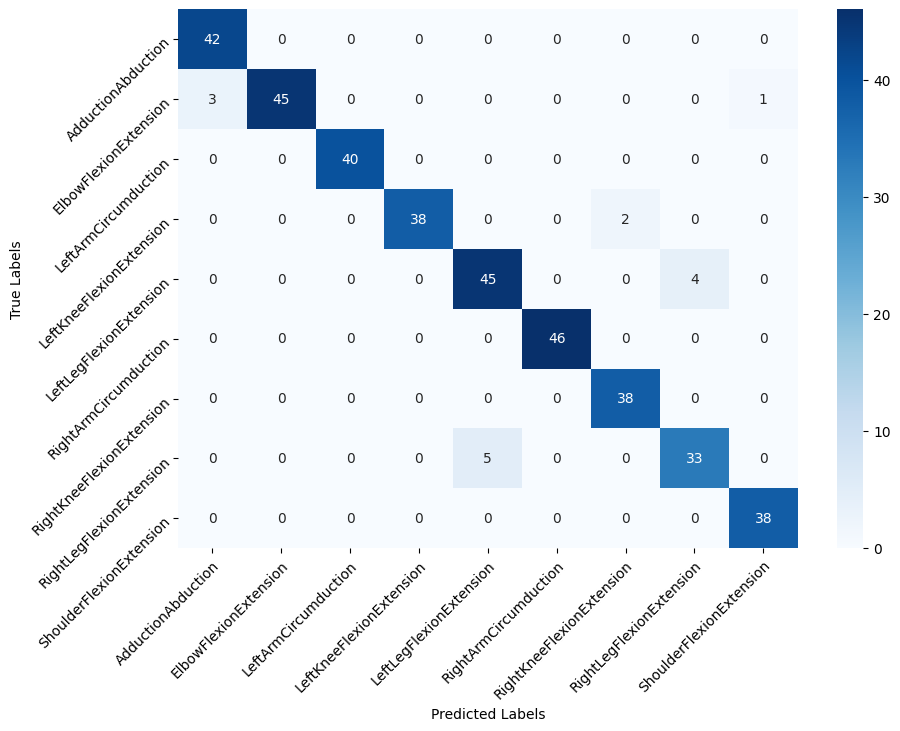
\includegraphics[width=1\textwidth]{bab4/ar_CNNLSTM_Confmatrix.png}
	\caption{Confusion matrix of the CNN-LSTM model outcomes.}
	\label{fig:CNNLSTM_Confmatrix}
\end{figure}

Figure \ref{fig:CNNLSTM_Confmatrix} displays the confusion matrix of the CNN-LSTM model. This confusion matrix illustrates the performance of the model in classifying various exercise activities for the elderly. The main diagonal shows the number of correct predictions for each class, while values off the main diagonal show the number of incorrect predictions.
% Gambar \ref{fig:CNNLSTM_Confmatrix} menampilkan confusion matrix model CNN-LSTM. Confusion matrix ini menggambarkan peforma model dalam mengklasifikasikan berbagai aktivitas latihan untuk lansia. Diagonal utama menunjukkan jumlah prediksi yang benar untuk setiap kelasnya, sementara nilai di luat diagonal utama menunjukkan jumlah prediksi yang salah.

Based on this matrix analysis, it appears that the model performs very well in classifying exercise activities for all classes. For example, the AdductionAbduction class, the model successfully predicted correctly 42 times without any errors. In addition to the AdductionAbduction class, there are other classes that were successfully predicted without any errors, i.e., LeftArmCircumduction, RightArmCircumduction, RightKneeFlexionExtension, and ShoulderFlexionExtension. The other class had some errors when the model tried to predict. For instance, 3 instances of the ElbowFlexionExtension class are considered as AdductionAbduction and 1 instance as ShoulderFlexionExtension. The RightLegFlexionExtension class has the highest error in prediction. Five instances are predicted as LeftLegFlexionExtension. Even so, this number of errors is still classified as a very low number of errors. The other class had some errors when the model tried to predict. For instance, 3 instances of the ElbowFlexionExtension class are considered as AdductionAbduction and 1 instance as ShoulderFlexionExtension. The RightLegFlexionExtension class has the highest error in prediction. Five instances are predicted as LeftLegFlexionExtension. Even so, this number of errors is still classified as a very low number of errors.
% Berdasarkan analisis matrix ini, tampak bahwa model memiliki peforma yang sangat baik dalam mengklasifikasikan aktifitas latihan untuk semua kelas. Sebagai contoh, kelas AdductionAbduction, model berhasil memprediksi dengan benar sebanyak 42 kali tanpa kesalahan. Meskipun ada beberapa kesalahan kecil, jumlah kesalahan ini tidak signifikan dan tidak mempengaruhi performa keseluruhan model secara drastis. Kesalahan prediksi ini menunjukkan bahwa model mungkin masih dapat ditingkatkan lebih lanjut, namun secara keseluruhan, model telah menunjukkan akurasi yang tinggi dan kemampuan generalisasi yang baik.

\begin{table}[h!]
	\centering
	\caption{Classification report of the CNN-LSTM model.}
	\label{tab:CNNLSTMreport}
	\begin{tabular}{rrrrr}
		\multicolumn{1}{l}{}      & precision            & recall               & f1-score             & support              \\
		\multicolumn{1}{l}{}      &                      &                      &                      &                      \\
		AdductionAbduction        & 0.93                 & 1.00                 & 0.97                 & 42                   \\
		ElbowFlexionExtension     & 1.00                 & 0.92                 & 0.96                 & 49                   \\
		LeftArmCircumduction      & 1.00                 & 1.00                 & 1.00                 & 40                   \\
		LeftKneeFlexionExtension  & 1.00                 & 0.95                 & 0.97                 & 40                   \\
		LeftLegFlexionExtension   & 0.90                 & 0.92                 & 0.91                 & 49                   \\
		RightArmCircumduction     & 1.00                 & 1.00                 & 1.00                 & 46                   \\
		RightKneeFlexionExtension & 0.95                 & 1.00                 & 0.97                 & 38                   \\
		RightLegFlexionExtension  & 0.89                 & 0.87                 & 0.88                 & 38                   \\
		ShoulderFlexionExtension  & 0.97                 & 1.00                 & 0.99                 & 38                   \\
		\multicolumn{1}{l}{}      & \multicolumn{1}{l}{} & \multicolumn{1}{l}{} & \multicolumn{1}{l}{} & \multicolumn{1}{l}{} \\
		accuracy                  &                      &                      & 0.96                 & 380                  \\
		macro avg                 & 0.96                 & 0.96                 & 0.96                 & 380                  \\
		weighted avg              & 0.96                 & 0.96                 & 0.96                 & 380
	\end{tabular}%
\end{table}

The classification report of the CNN-LSTM model is shown in table \ref{tab:CNNLSTMreport}. This table includes several metrics, i.e., precision, recall, f1-score, and support for each class. In addition, the overall value of the model is also displayed using macro averaging and weighted averaging methods. There are several classes that have perfect precision values (1.00). These classes are ElbowFlexionExtension, LeftArmCircumduction, LeftKneeFlexionExtension, and RightArmCircumduction. This value indicates that the model correctly predicted all instances of these classes. This result is in line with the explanation in the previous confusion matrix. Although not perfect, the other classes have high precision values too. The lowest precision value in this model is in the RightLegFlexionExtension class of 0.89. This value is high considering that in previous models there were several classes with lower precision values. In another metric, recall, the model is able to predict finding all positive instances very well. There are 4 classes with perfect recall values, namely AdductionAbduction, LeftArmCircumduction, RightArmCircumduction, RightKneeFlexionExtension and ShoulderFlexionExtension. Similar to precision, the lowest recall value in this model is 0.87, in the RightLegFlexionExtension and RightLegFlexionExtension classes.
% Penjelasan classification report model CNN-LSTM ditunjukkan pada tabel \ref{tab:CNNLSTMreport}. Tabel ini mencakup beberapa metris, yaitu precision, recall, f1-score, dan support untuk setiap kelasnya. Selain itu, nilai keseluruhan dari model juga ditampilkan menggunakan metode macro averaging dan weighted averaging. Terdapat beberapa kelas yang memiliki nilai precision sempurna (1.00). Kelas-kelas tersebut adalah AdductionAbduction, LeftArmCircumduction, RightKneeFlexionExtension, dan ShoulderFlexionExtension. Nilai ini menunjukkan model berhasil memprediksi dengan benar seluruh instance pada kelas tersebut. Hasil ini selaras dengan penjelasan pada confusion matrix sebelumnya. Meskipun tidak sempurna, kelas lainnya memiliki nilai precision yang tinggi juga. Nilai precision terendah pada model ini berada pada kelas RightLegFlexionExtension sebesar 0.97. Nilai ini termasuk tinggi mengingat pada model-model sebelumnya terdapat beberapa kelas dengan nilai precision lebih rendah. Pada metric yang lain, yaitu recall, model mampu memprediksi menemukan semua instance positif dengan sangat baik. Terdapat 4 kelas dengan nilai recall sempurna, yaitu AdductionAbduction, LeftArmCircumduction, LeftKneeFlexionExtension, dan ShoulderFlexionExtension. Sama halnya dengan precision, nilai recall terendah pada model ini adalah 0.97, pada kelas RightKneeFlexionExtension dan RightLegFlexionExtension.

F1-score shows the average harmony between precision and recall. Similar to the previous two metrics, the f1-score of each class in this model shows satisfactory results. The lowest value in this metric is 0.88 and is only in one class, namely RightLegFlexionExtension. There are 2 classes with perfect f1-score values, namely LeftArmCircumduction, and RightArmCircumduction. This perfect F1-score is obtained from perfect results in the precision and recall of these classes. Both macro averaging and weighted averaging, the average value of all metrics for this model is at a very high value. For all metrics, the score was 0.96 for both methods. These results show excellent performance in all classes whether or not the data distribution is taken into account.
% F1-score menunjukkan rata-rata keharmonisan antara precision dan recall. Sama halnya dengan 2 metric sebelumnya, f1-score setiap kelas pada model ini menunjukkan hasil yang memuaskan. Nilai terendah pada metric ini adalah 0.97 dan hanya berada pada satu kelas saja, yaitu RightLegFlexionExtension. Terdapat 3 kelas dengan nilai f1-score sempurna, yaitu AdductionAbduction, LeftArmCircumduction, dan ShoulderFlexionExtension. F1-score yang sempurna ini didapatkan dari hasil yang sempurna juga pada precision dan recall kelas-kelas tersebut. Baik macro averaging maupun weighted averaging, nilai rata-rata seluruh metric untuk model ini berada pada nilai yang sangat tinggi. Untuk seluruh metrics mendapatkan nilai sebesar 0.99 pada kedua metode ini. Hasil ini menunjukkan peforma yang sangat baik di semua kelas baik memperhitungkan distribusi data yang ada maupun tidak.

\begin{table}[h!]
	\caption{Accuracy results for training, validation, and test data of the CNN-LSTM model.}
	\label{tab:CNNLSTMAccuracy}
	\centering
	\begin{tabular}{|c|c|c|}
		\hline
		Training accuracy (\%) & Validation accuracy (\%) & Test accuracy (\%) \\ \hline
		96.71                  & 96.04                    & 96.05              \\ \hline
	\end{tabular}
\end{table}

Another measurement calculated is the accuracy value of the model against the training, validation, and test data. Table \ref{tab:CNNLSTMAccuracy} shows the accuracy value of each data. The training accuracy shows a high result of 96.71\%. This high accuracy shows that the model is able to learn the training data patterns very well. The learning error is very small. On the validation data, the accuracy was 96.04\%. This high value has shown that the model is not just overfitting the training data. The model was able to classify the new data very well. This training and validation accuracy value is consistent with the previous graph which shows an increase in accuracy every epoch. Model testing was performed on completely new data using test data. The test accuracy that emerged in this model was 96.05\%. The very high accuracy on all data confirms that the model is reliable and has good generalization.
% Pengukuran lain yang dihitung adalah nilai akurasi model terhadap data latih, validasi, dan uji. Tabel \ref{tab:CNNLSTMAccuracy} menunjukkan nilai akurasi setiap datanya. Akurasi pelatihan menunjukkan hasil yang tinggi, yaitu 99.67\%. Akurasi yang tinggi ini menunjukkan bahwa model mampu mempelajari pola data pelatihan dengan sangat baik. Kesalahan pembelajaran yang terjadi begitu kecil. Pada data validasi, akurasi yang muncul sebesar 98.68\%. Nilai yang tinggi ini telah menunjukkan bahwa model tidak hanya melakukan overfitting pada data pelatihan. Model mampu mengklasifikasikan data baru dengan sangat baik. Nilai akurasi pelatihan dan validasi ini konsisten dengan grafik sebelumnya yang menunjukkan peningkatan akurasi setiap epochnya. Pengujian model dilakukan pada data yang benar-benar baru menggunakan data uji. Akurasi uji yang muncul pada model ini sebesar 98.68\%. Akurasi yang sangat tinggi pada seluruh data menegaskan 	bahwa model dapat diandalkan dan memiliki generalisasi yang baik.

\subsection{Deep CNN-LSTM Model Performance}
\label{subsec4:DeepCNNLSTMPerformance}

\begin{figure}[h!]
	\centering
	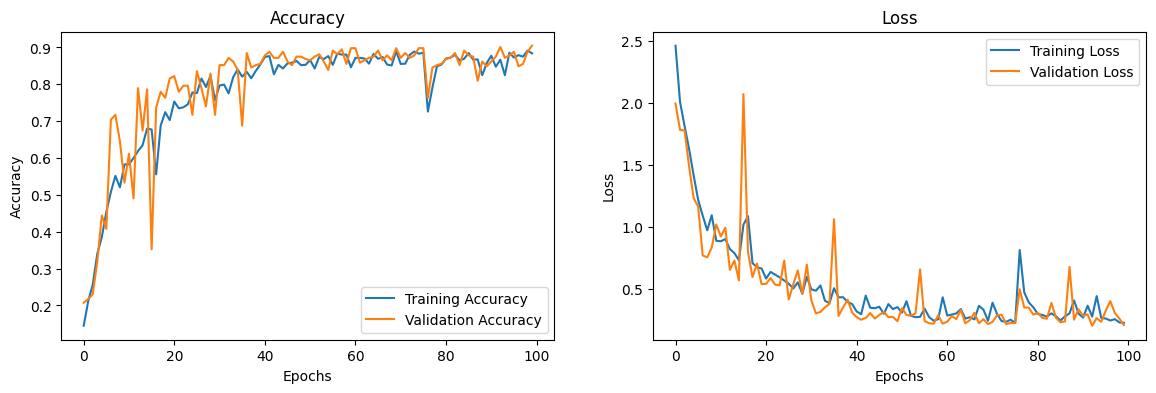
\includegraphics[width=1\textwidth]{bab4/ar_DeepCNNLSTM_AccLoss.png}
	\caption{Accuracy and loss of training and validation on the Deep CNN-LSTM model.}
	\label{fig:DeepCNNLSTM_AccLoss}
\end{figure}

The next architecture used for training the PhysioExercise dataset is deep CNN-LSTM. This training resulted in a deep CNN-LSTM model. Figure \ref{fig:DeepCNNLSTM_AccLoss} shows a detailed overview of the accuracy and loss for each epoch. There are two lines representing the training and validation data. The training took place in 100 epochs. The training accuracy of each epoch has a good increase. The gradual increase from the beginning to the end of training shows the ability of the model to learn and adapt to the given data pattern. Fluctuations occur in the training data, but the fluctuations are not too large. Unlike the validation accuracy, which experienced high fluctuations on several occasions. Even so, the trend of validation data shows the same trend as training accuracy. Both go hand in hand in improving the model's ability to learn data patterns.
% Arsitektur berikutnya yang digunakan untuk pelatihan dataset PhysioExercise adalah deep CNN-LSTM. Pelatihan ini menghasilkan sebuah model deep CNN-LSTM. Gambar \ref{fig:DeepCNNLSTM_AccLoss} menunjukkan gambaran detail akurasi dan loss setiap epochnya. Terdapat dua garis yang merepresentasikan data latih dan validasi. Pelatihan berlangsung dalam 100 epoch. Akurasi pelatihan setiap epochnya mengalami kenaikan yang baik. Kenaikan bertahap sejak awal hingga akhir pelatihan menunjukkan kemampuan model dalam mempelajari dan beradaptasi dengan pola data yang diberikan. Fluktuasi terjadi pada data pelatihan, namun fluktuasi yang terjadi tidak terlalu besar. Berbeda dengan akurasi validasi yang mengalami fluktuasi cukup tinggi dibeberapa kesempatan. Meskipun begitu, tren yang dimiliki data validasi menunjukkan tren yang sama dengan akurasi pelatihan. Keduanya beriringan dalam peningkatan kemampuan model mempelajari pola data.

The loss graph illustrates the decrease in loss values on the training and validation datasets. The decreasing value indicates that the model is able to reduce errors in learning data patterns. Entering the 41st epoch, the loss values in both training and validation experience values that tend to stabilize towards lower values. Even so, fluctuations in both losses occurred during the training process. Especially in the validation data, the loss value had a fairly high spike at some points. This spike was quite high at the beginning of the training. The spike indicates that the model had experienced some overfitting because it relied too much on the training data.
% Grafik loss menggambarkan penurunan nilai loss pada dataset pelatihan dan validasi. Nilai yang semakin menurun menunjukkan model mampu mengurangi kesalahan dalam mempelajari pola data. Loss terus mengalami penurunan hingga pada epoch ke 40. Memasuki epoch ke 41, nilai loss pada pelatihan maupun validasi mengalami nilai yang cenderung stabil menuju pada nilai yang lebih rendah. Meskipun begitu, fluktuasi pada kedua loss terjadi selama proses pelatihan berlangsung. Terutama pada data validasi, nilai loss sempat mengalami lonjakan yang cukup tinggi di beberapa titik. Lonjakan ini cukup tinggi pada awal-awal pelatihan. Kondisi lonjakan yang naik menunjukkan model sempat mengalami beberapa kali overfitting karena terlalu bertumpu pada data pelatihan. 

\begin{figure}[h!]
	\centering
	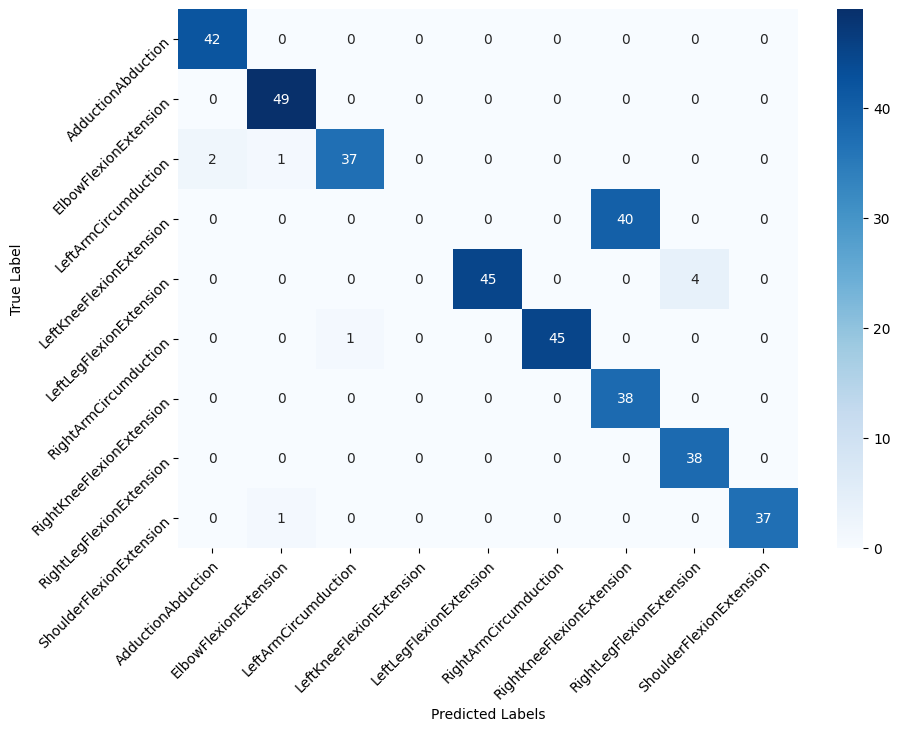
\includegraphics[width=1\textwidth]{bab4/ar_DeepCNNLSTM_Confmatrix.png}
	\caption{Confusion matrix of the Deep CNN-LSTM model outcomes.}
	\label{fig:DeepCNNLSTM_Confmatrix}
\end{figure}

Figure \ref{fig:DeepCNNLSTM_Confmatrix} displays the prediction results of the deep CNN-LSTM model against each class. The main diagonal shows the number of correct predictions for each class. While the values on the off-diagonal show the number of incorrect predictions. Overall, the model has a good ability to predict each instance. For example, the model successfully classified 42 AdductionAbduction samples, 49 ElbowFlexionExtension samples, 38 RightKneeFlexionExtension samples, and 38 RightLegFlexionExtension samples without any error.
% Gambar \ref{fig:DeepCNNLSTM_Confmatrix} menampilkan hasil prediksi model deep CNN-LSTM terhadap masing-masing kelas. Diagonal utama menunjukkan jumlah prediksi benar dari setiap kelasnya. Sedangkan nilai pada off-diagonal menunjukkan jumlah prediksi yang salah. Secara keseluruhan, model memiliki kemampuan yang baik dalam memprediksi setiap instance yang ada. Sebagai contoh, model berhasil mengklasifikasikan 42 sampel AdductionAbduction, 49 sampel ElbowFlexionExtension, 38 sampel RightKneeFlexionExtension, dan 38 sampel RightLegFlexionExtension tanpa kesalahan sama sekali. 

There was one class where the model failed to correctly predict all instances, namely the LeftKneeFlexionExtension class. Of all the instances, instead of predicting it as the LeftLegFlexionExtension class, the model predicted it as RightKneeFlexionExtension. This is a very likely error given that these two classes have similar motion spaces. In the remaining instances, the misclassification was minor and insignificant. The features of the two classes are also similar, so the model experiences confusion in classifying correctly. In addition, when looking back at the dataset, the angle of the image capture needs to be paid more attention so that the keypoint extraction process becomes better. The addition of augmentation data is important if the model is not good enough to classify all classes.
% Terdapat satu kelas dimana model gagal memprediksi dengan benar seluruh instance, yaitu kelas LeftKneeFlexionExtension. Dari seluruh instance yang ada, alih-alih memprediksi sebagai kelas LeftLegFlexionExtension, model justru memprediksi sebagai RightKneeFlexionExtension. Kesalahan sangat mungkin terjadi mengingat kedua kelas ini memiliki ruang gerak yang mirip. Fitur yang dimilki kedua kelas juga mirip, sehingga model mengalami kebingungan dalam mengklasifikasikan secara benar. Selain itu apabila melihat kembali dataset, sudut pengambilan gambar perlu lebih diperhatikan agar dalam proses ekstraksi keypoint menjadi lebih baik. Penambahan data augmentasi menjadi penting apabila model yang digunakan tidak cukup baik dalam mengklasifikasikan seluruh kelas.

The classification report of the deep CNN-LSTM model is presented in table \ref{tab:DeepCNNLSTMreport}. Evaluation using the classification report shows the precision, recall, and F1-score metrics for each activity. This classification model has shown quite good performance. Overall, the accuracy of the model was 0.87. The overall results for each metric were calculated using macro averaging and weighted averaging methods. Using macro averaging, the average results for precision, recall, and F1-score of this model are 0.81, 0.87, 0.83 respectively. Unlike the macro averaging method, calculations using the weighted averaging method showed a precision of 0.82, recall of 0.87, and F1-score of 0.84. This method is more representative of the class distribution in a dataset.
% Classification report model deep CNN-LSTM disajikan pada tabel \ref{tab:DeepCNNLSTMreport}. Evaluasi menggunakan classification report menunjukkan metris precision, recall, dan F1-score untuk setiap aktifitas. Model klasifikasi ini telah menunjukkan peforma yang cukup baik. Secara keseluruhan, akurasi model ini sebesar 87\%. Hasil keseluruhan pada setiap metrisnya dihitung menggunakan metode macro averaging dan weighted averaging. Menggunakan macro averaging, hasil rata-rata untuk precision, recall, dan F1-score model ini sebesar 0.81, 0.87, 0.83 respectively. Berbeda dengan metode macro averaging, perhitungan menggunakan metode weighted averaging menunjukkan hasil precision sebesar 0.82, recall sebesar 0.87, dan F1-score sebesar 0.84. Metode ini lebih representatif terhadap distribusi kelas dalam sebuah dataset.

\begin{table}[h!]
	\centering
	\caption{Classification report of the Deep CNN-LSTM model.}
	\label{tab:DeepCNNLSTMreport}
	\begin{tabular}{rrrrr}
		\multicolumn{1}{l}{}      & precision            & recall               & f1-score             & support              \\
		\multicolumn{1}{l}{}      &                      &                      &                      &                      \\
		AdductionAbduction        & 0.95                 & 1.00                 & 0.98                 & 42                   \\
		ElbowFlexionExtension     & 0.96                 & 1.00                 & 0.98                 & 49                   \\
		LeftArmCircumduction      & 0.97                 & 0.93                 & 0.95                 & 40                   \\
		LeftKneeFlexionExtension  & 0.00                 & 0.00                 & 0.00                 & 40                   \\
		LeftLegFlexionExtension   & 1.00                 & 0.92                 & 0.96                 & 49                   \\
		RightArmCircumduction     & 1.00                 & 0.98                 & 0.99                 & 46                   \\
		RightKneeFlexionExtension & 0.49                 & 1.00                 & 0.66                 & 38                   \\
		RightLegFlexionExtension  & 0.90                 & 1.00                 & 0.95                 & 38                   \\
		ShoulderFlexionExtension  & 1.00                 & 0.97                 & 0.99                 & 38                   \\
		\multicolumn{1}{l}{}      & \multicolumn{1}{l}{} & \multicolumn{1}{l}{} & \multicolumn{1}{l}{} & \multicolumn{1}{l}{} \\
		accuracy                  &                      &                      & 0.87                 & 380                  \\
		macro avg                 & 0.81                 & 0.87                 & 0.83                 & 380                  \\
		weighted avg              & 0.82                 & 0.87                 & 0.84                 & 380
	\end{tabular}%
\end{table}

The precision value measures the correct positive predictions out of all positive predictions made by the model. A higher precision indicates the model makes fewer errors in predicting a particular class. Based on the table \ref{tab:DeepCNNLSTMreport}, there are several classes with perfect precision values. The classes are LeftLegFlexionExtension, RightArmCircumduction, and ShoulderFlexionExtension. For the other classes, the model has a good ability to predict the given instance. However, there is one class with a very low precision value, namely RightKneeFlexionExtension. Precision in this class is only 0.49. This fairly low value indicates the number of instances that are predicted incorrectly by the model. In addition, there is one class where the model failed to predict correctly. That class is LeftKneeFlexionExtension. The precision value of 0.00 indicates that the model did not predict this class correctly at all. This precision value is in line with the discussion on the confusion matrix for the LeftKneeFlexionExtension class.
% Nilai precision mengukur prediksi positif yang benar dari keseluruhan prediksi positif yang dibuat oleh model. Precision yang semakin tinggi menunjukkan model membuat sedikit kesalahan dalam memprediksi kelas tertentu. Berdasarkan tabel \ref{tab:DeepCNNLSTMreport}, terdapat beberapa kelas dengan nilai precision sempurna. Kelas yang dimaksudkan adalah LeftLegFlexionExtension, RightArmCircumduction, dan ShoulderFlexionExtension. Terhadap kelas yang lain, model memiliki kemampuang yang baik dalam memprediksi instance yang diberikan. Namun, terdapat satu kelas dengan nilai precision sangat rendah, yaitu RightKneeFlexionExtension. Precision pada kelas ini hanya 0.49. Nilai yang cukup rendah ini menunjukkan banyaknya instance yang diprediksi salah oleh model. Selain itu, terdapat satu kelas dimana model gagal dalam memprediksi dengan benar. Kelas tersebut adalah LeftKneeFlexionExtension. Nilai precision 0.00 menujukkan model tidak sama sekali memprediksi dengan benar pada kelas ini. Nilai precision ini selaras dengan pembahasan pada confusion matrix untuk kelas LeftKneeFlexionExtension. 

Similar to precision, the recall results for some classes have perfect values. These classes are AdductionAbduction, ElbowFlexionExtension, RightKneeFlexionExtension, and RightLegFlexionExtension. This value indicates the model's good ability to find predictions for all positive instances. In the case of the RightKneeFlexionExtension class, the recall value of this class is not as bad as the precision value. Precision is quite low despite perfect recall, indicating that many predictions are wrong for this class. In the other hand, the LeftKneeFlexionExtension class gets no recall value at all, which is 0.00. In the other metric, f1-score, every class is above 0.90 except for two classes. The two classes are RightKneeFlexionExtension and LeftKneeFlexionExtension. The RightKneeFlexionExtension class had an f1-score of 0.66. This is far below the f1-score of the other classes. Even worse, the LeftKneeFlexionExtension class does not get an f1-score at all. This is related to the absence of precision and recall values for this class. The model failed to predict this class. One of the reasons is the complexity of this movement.
% Sama halnya dengan precision, hasil recall pada beberapa kelas memiliki nilai yang sempurna. Kelas-kelas tersebut adalah AdductionAbduction, ElbowFlexionExtension, RightKneeFlexionExtension, dan RightLegFlexionExtension. Nilai ini menunjukkan kemampuan baik model dalam menemukan prediksi seluruh instance positif. Pada kasus kelas RightKneeFlexionExtension, nilai recall kelas ini tidak seburuk nilai precisionnya. Precision cukup rendah meskipun recall sempurna, menunjukkan bahwa banyak prediksi yang salah untuk kelas ini. In the other hand, kelas LeftKneeFlexionExtension tidak mendapatkan nilai recall sama sekali, yaitu 0.00. Pada metric yang lain, yaitu f1-score, nilai setiap kelasnya berada di atas 0.90 kecuali dua kelas. Kedua kelas tersebut adalah RightKneeFlexionExtension dan LeftKneeFlexionExtension. Kelas RightKneeFlexionExtension mendapatkan f1-score sebesar 0.66. Nilai ini berada jauh d bawah nilai f1-score kelas lainnya. Lebih parah lagi, kelas LeftKneeFlexionExtension tidak mendapatkan nilai f1-score sama sekali. Hal ini berkaitan dengan tidak adanya nilai precision dan recall pada kelas ini. Model gagal memprediksi kelas ini. Salah satu alasannya adalah kompleksitas pada gerakan ini. 

The overall results for each metric were calculated using macro averaging and weighted averaging methods. Using macro averaging, the average results for precision, recall, and F1-score of this model are 0.81, 0.87, and 0.83 respectively. Unlike the macro averaging method, calculations using the weighted averaging method showed a precision of 0.82, recall of 0.87, and F1-score of 0.84. The macro average and weighted average of precision, recall, and F1-Score each show good values, indicating a balanced performance in most classes.
% Hasil keseluruhan pada setiap metrisnya dihitung menggunakan metode macro averaging dan weighted averaging. Menggunakan macro averaging, hasil rata-rata untuk precision, recall, dan F1-score model ini sebesar 0.81, 0.87, dan 0.83 respectively. Berbeda dengan metode macro averaging, perhitungan menggunakan metode weighted averaging menunjukkan hasil precision sebesar 0.82, recall sebesar 0.87, dan F1-score sebesar 0.84. Rata-rata makro dan rata-rata terbobot dari precision, recall, dan F1-Score masing-masing menunjukkan nilai yang baik, mengindikasikan performa yang seimbang di sebagian besar kelas. 

\begin{table}[h!]
	\caption{Accuracy results for training, validation, and test data of the deep CNN-LSTM model.}
	\label{tab:DeepCNNLSTMAccuracy}
	\centering
	\begin{tabular}{|c|c|c|}
		\hline
		Training accuracy (\%) & Validation accuracy (\%) & Test accuracy (\%) \\ \hline
		89.14                  & 90.43                    & 87.11              \\ \hline
	\end{tabular}
\end{table}

Figure \ref{tab:DeepCNNLSTMAccuracy} provides information about the accuracy of the deep CNN-LSTM model on training data, validation data, and test data. This is the final part of the evaluation series that has previously been illustrated through the accuracy and loss graphs, confusion matrix, and classification report. The model achieved an accuracy of 89.14\% on the training data. This shows that the model is able to learn from the training data quite well, identifying patterns that match the target. The accuracy on the validation data reached 90.43\%. The higher accuracy on the validation data compared to the training data indicates that the model has good generalization ability and is not overfitting on the training data. The accuracy on the test data was 87.11\%. This is the most important metric as it describes the performance of the model on data that is completely new and not seen during training and validation. This accuracy is consistent with the validation accuracy and slightly lower, which is still within reasonable limits, indicating that the model is reliable in making predictions on new data.
% Gambar \ref{tab:DeepCNNLSTMAccuracy} memberikan informasi mengenai akurasi model deep CNN-LSTM pada data latih, data validasi, dan data uji. Ini adalah bagian akhir dari rangkaian evaluasi yang sebelumnya telah diilustrasikan melalui grafik akurasi dan loss, confusion matrix, dan classification report. Model mencapai akurasi sebesar 89.14\% pada data latih. Ini menunjukkan bahwa model mampu belajar dari data pelatihan dengan cukup baik, mengidentifikasi pola yang sesuai dengan target. Akurasi pada data validasi mencapai 90.43\%. Akurasi yang lebih tinggi pada data validasi dibandingkan dengan data latih menunjukkan bahwa model memiliki kemampuan generalisasi yang baik dan tidak overfitting pada data pelatihan. Akurasi pada data uji adalah 87.11\%. Ini adalah metrik yang paling penting karena menggambarkan kinerja model pada data yang benar-benar baru dan tidak terlihat selama pelatihan dan validasi. Akurasi ini konsisten dengan akurasi validasi dan sedikit lebih rendah, yang masih dalam batas wajar, menunjukkan bahwa model dapat diandalkan dalam membuat prediksi pada data baru.


\section{Performance Analysis of Models}
\label{sec:ModelAnalysis}

There are 4 different models that have been generated in this work. These models have different architectures used. An in-depth discussion has been done in the previous section. The results of the four models were then analyzed to compare the performance of each model. Table \ref{tab:ComparisonTable} shows an overview of the performance of each model. Several metrics are taken for comparison. These metrics are precision, recall, f1-score, accuracy, and model loss.
% Terdapat 4 model berbeda yang telah dihasilkan pada pekerjaan ini. Model-model ini memiliki berbedaan arsitektur yang digunakan. Pembahasan mendalam telah dilakukan pada bagian sebelumnya. Hasil dari keempatnya kemudian dianalisis untuk dibandingkan peforma masing-masing model. Tabel \ref{tab:ComparisonTable} menunjukkan overview dari peforma setiap modelnya. Beberapa metric diambil untuk dibandingkan. Metric-metric tersebut adalah precision, recall, f1-score, accuracy, dan loss model.

\begin{table}[h!]
	\caption{Classification performance of exercise activities for the elderly on models.}
	\label{tab:ComparisonTable}
	\centering
	\begin{tabular}{|cl|r|r|r|r|}
		\hline
		\multicolumn{2}{|c|}{Metrics}                                                                     & \multicolumn{1}{c|}{CNN} & \multicolumn{1}{c|}{LSTM} & \multicolumn{1}{c|}{CNN-LSTM} & \multicolumn{1}{c|}{\begin{tabular}[c]{@{}c@{}}Deep \\ CNN-LSTM\end{tabular}}        \\ \hline
		\multicolumn{1}{|c|}{\multirow{3}{*}{\begin{tabular}[c]{@{}c@{}}Macro\\ Average\end{tabular}}}    & Precision                & 0.85                      & 0.93                          & \textbf{0.96}                                                                 & 0.81 \\ \cline{2-6}
		\multicolumn{1}{|c|}{}                                                                            & Recall                   & 0.83                      & 0.93                          & \textbf{0.96}                                                                 & 0.87 \\ \cline{2-6}
		\multicolumn{1}{|c|}{}                                                                            & F1-Score                 & 0.81                      & 0.93                          & \textbf{0.96}                                                                 & 0.83 \\ \hline
		\multicolumn{1}{|c|}{\multirow{3}{*}{\begin{tabular}[c]{@{}c@{}}Weighted\\ Average\end{tabular}}} & Precision                & 0.86                      & 0.94                          & \textbf{0.96}                                                                 & 0.82 \\ \cline{2-6}
		\multicolumn{1}{|c|}{}                                                                            & Recall                   & 0.84                      & 0.93                          & \textbf{0.96}                                                                 & 0.87 \\ \cline{2-6}
		\multicolumn{1}{|c|}{}                                                                            & F1-Score                 & 0.82                      & 0.93                          & \textbf{0.96}                                                                 & 0.84 \\ \hline
		\multicolumn{2}{|l|}{Accuracy (\%)}                                                               & 83.68                    & 92.89                     & \textbf{96.05}                & 87.11                                                                                \\ \hline
		\multicolumn{2}{|l|}{Loss}                                                                        & 0.4513                   & 0.2629                    & \textbf{0.1498}               & 0.3004                                                                               \\ \hline
	\end{tabular}
	\caption*{Higher is better. For loss, lower is better.}
\end{table}

The model performance comparison table shows that the CNN-LSTM architecture consistently has the best performance in the classification of exercise activities for the elderly compared to the CNN, LSTM, and Deep CNN-LSTM models. The CNN model is the model with the lowest performance. The accuracy value of this model is only 83.68\% and the loss value is quite high, which is 0.4513. The Deep CNN-LSTM model is the next low-performing model. The accuracy of this model is at 87.11\% with a loss value of 0.3004. Unlike the two previous models, the LSTM model has a better performance. The accuracy of this model is at a value of 92.89\% and the loss is 0.2629. The CNN-LSTM model is the model with the best performance. The accuracy of the CNN-LSTM model is 96.05\% and the loss is 0.1498. This figure shows the ability of the CNN-LSTM model in the classification work of the best exercise activity compared to other models.
% Tabel perbandingan performa model menunjukkan bahwa arsitektur CNN-LSTM secara konsisten memiliki performa terbaik dalam klasifikasi aktivitas latihan untuk elderly dibandingkan dengan model CNN, LSTM, dan Deep CNN-LSTM. Model CNN menjadi model dengan peforma paling rendah. Nilai akurasi model ini hanya 83.68% dan nilai loss yang cukup tinggi, yaitu 0.4513. Model Deep CNN-LSTM menjadi model dengan peforma rendah berikutnya. Akurasi model ini berada pada nilai 87.11% dengan loss bernilai 0.3004. Berbeda dengan kedua model sebelumnya, model LSTM memiliki peforma yang lebih baik. Akurasi model ini berada pada nilai 92.89% dan loss bernilai 0.2629. Model CNN-LSTM menjadi model dengan peforma paling baik. Akurasi model CNN-LSTM bernilai 96.05% dan loss 0.1498. Angka ini menunjukkan kemampuan model CNN-LSTM dalam pekerjaan klasifikasi aktifitas latihan paling baik dibandingkan model lainnya.

% bagian CNN
The CNN model is the model with the worst performance compared to other models. The accuracy of this model is only 83.68\%. This figure shows that the accuracy of the model in classifying exercise activities is very low. In the classification process, the CNN model has the highest error rate among other models. This is indicated by the highest loss value of the CNN model compared to other models. CNN model loss is 0.4513. There are many factors that can affect the low performance of the CNN model. CNN is a well-known architecture in the context of image data processing. In time series data processing, the time series data structure will be considered as a one-dimensional image. This data structure will consider time as one dimension and other features as other dimensions. However, CNN's ability to handle this data has many limitations. CNNs tend to be less effective in capturing long-term dependencies in time series data, especially when compared to LSTM. In addition, determining the right CNN architecture for time series is a job in itself because it is more complicated when compared to other architectures such as LSTM. The dataset used in this work is a time series data with a large number of windows and features. With the large amount of temporal and spatial data used, the CNN model did not succeed in classifying the instances properly.
% Model CNN menjadi model dengan peforma paling buruk dibandingkan dengan model lainnya. Akurasi model ini hanya bernilai 83.68\%. Angka ini menunjukkan tingkat ketepatan model dalam mengklasifikasikan aktifitas latihan sangat rendah. Dalam proses klasifikasi, model CNN memiliki tingkat kesalahan paling tinggi diantara model lainnya. Hal ini ditunjukkan dengan nilai loss model CNN tertinggi dibandingkan dengan model lainnya. Loss model CNN bernilai 0.4513. Terdapat banyak faktor yang dapat mempengaruhi peforma model CNN yang rendah ini. CNN merupakan arsitektur yang dikenal dalam konteks pengolahan data citra. Dalam pengolahan data time series, struktur data time series akan dianggap sebagai citra satu dimensi. Struktur data ini akan menganggap waktu sebagai satu dimensi dan fitur lainnya sebagai dimensi lainnya. Akan tetapi, kemampuan CNN dalam menangani data ini memiliki banyak batasan. CNN cenderung kurang efektif dalam menangkap dependensi jangka panjang dalam data time series, terutama apabila dibandingkan dengan LSTM. Selain itu, penentuan arsitektur CNN yang tepat untuk time series menjadi pekerjaan tersendiri karena lebih rumit apabila dibandingkan dengan arsitektur lainnya seperti LSTM. Dataset yang digunakan pada pekerjaan ini merupakan data time series dengan jumlah window dan fitur yang cukup banyak. Dengan banyaknya data temporal dan spasial yang digunakan, model CNN tidak berhasil melakukan klasifikasi instance dengan baik.

% bagian LSTM
The performance of the LSTM model is high compared to the CNN and Deep CNN-LSTM models. The LSTM model used in the classification of exercise activities in the elderly showed excellent performance, with high accuracy on training, validation, and test data. The accuracy-loss graph shows a steady and consistent upward trend, while the confusion matrix and classification report provide further evidence of the model's ability to correctly classify most classes. However, the model is not better when compared to the CNN-LSTM model. LSTM models are designed to capture long-term temporal dependencies, but are not effective in extracting locally or spatially significant features in short time windows. In the dataset used, the spatial data in question is the keypoint extracted features from the Mediapipe framework. The LSTM model is not able to handle this keypoint extraction data compared to the CNN-LSTM model. The LSTM model is a complex model with many parameters that can cause overfiting problems. In addition, the LSTM model requires a lot of data for effective training. In contrast to the CNN-LSTM model, where CNN will reduce the dimensions of the input entering the LSTM. In the end, the complexity of the CNN-LSTM model becomes lower and is able to improve generalization.
% Peforma model LSTM tergolong tinggi dibandingkan dengan model CNN dan Deep CNN-LSTM. Model LSTM yang digunakan dalam klasifikasi aktivitas latihan pada elderly menunjukkan performa yang sangat baik, dengan akurasi tinggi pada data pelatihan, validasi, dan uji. Grafik akurasi-loss menunjukkan tren peningkatan yang stabil dan konsisten, sementara confusion matrix dan classification report memberikan bukti lebih lanjut tentang kemampuan model dalam mengklasifikasikan sebagian besar kelas dengan benar. Meskipun begitu, model ini tidak lebih baik apabila dibandingkan dengan model CNN-LSTM. Model LSTM dirancang untuk menangkap dependensi temporal jangka panjang, namun tidak efektif dalam mengekstraksi fitur lokal atau spasial yang signifikan dalam jendela waktu yang pendek. Pada dataset yang digunakan, data spasial yang dimaksud adalah fitur ekstraksi keypoint dari framework Mediapipe. Model LSTM tidak mampu menangani data ekstraksi keypoint ini dibandingkan dengan model CNN-LSTM. Model LSTM merupakan model yang kompleks dengan banyaknya parameter yang dapat menyebabkan masalah overfiting. Selain itu, model LSTM memerlukan banyak data untuk pelatihan yang efektif. Berbeda dengan model CNN-LSTM, dimana CNN akan mereduksi dimensi input yang masuk ke LSTM. Pada akhirnya kompleksitas model CNN-LSTM menjadi lebih rendah dan mampu meningkatkan generalisasi.

% tambahan bagian LSTM
% LSTM cenderung lebih lambat dalam pelatihan dan inferensi dibandingkan CNN karena sifat sekuensialnya yang sulit untuk diparalelkan. CNN berperan dalam mereduksi dimensi, dimana inferensi menjadi lebih cepat. LSTM mungkin tidak sepenuhnya memanfaatkan struktur data 2D atau 3D yang ada dalam data keypoint, karena lebih berfokus pada urutan temporal. CNN membantu dalam ekstraksi di awal, sehingga mengurangi kebutuhan akan jumlah parameter yang besar dalam LSTM. 

% bagian CNN-LSTM
CNN-LSTM achieved the highest precision, recall, and f1-score values in both macro average and weighted average metrics, with 0.96 each. This shows that the CNN-LSTM model is highly accurate in making positive predictions and is able to detect almost all positive instances correctly, providing an optimal balance between precision and recall. In addition, the CNN-LSTM model also showed the highest accuracy of 96.05\% and the lowest loss value of 0.1498, reflecting a very low prediction error rate. The combination of CNN and LSTM shows a good ability to handle spatial data and temporal data in one dataset.
% CNN-LSTM mencapai nilai precision, recall, dan f1-score tertinggi baik dalam metrik macro average maupun weighted average, dengan masing-masing sebesar 0.99. Hal ini menunjukkan bahwa model CNN-LSTM sangat akurat dalam membuat prediksi positif dan mampu mendeteksi hampir semua instance positif dengan benar, memberikan keseimbangan yang optimal antara precision dan recall. Selain itu, model CNN-LSTM juga menunjukkan akurasi tertinggi sebesar 98.68\% dan nilai loss terendah sebesar 0.0683, yang mencerminkan tingkat kesalahan prediksi yang sangat rendah. Kombinasi CNN dan LSTM menunjukkan kemampuan yang baik dalam menangani data spasial dan data temporal dalam satu dataset. 

% bagian Deep CNN-LSTM
The Deep CNN-LSTM model is a model with poor performance after the CNN model. This model has a similar architecture to the CNN-LSTM model. The difference of this model is the addition of several CNN layers that become deeper in the training process. However, the additional layer architecture does not show better results. There are several reasons why this might happen. First, too many layers make the model learn too much from the training data and fail to generalize to the test data. This is evidenced in the figure \ref{fig:DeepCNNLSTM_AccLoss} where the accuracy of the validation dta experiences many times large fluctuations. Secondly, more complex models require more data to train effectively. If the available data is not large enough or diverse enough, adding layers is ineffective because it does not have enough information to learn the data patterns. This will create a model that needs to be. Thirdly, the addition of these layers causes redundancy in the extracted features. Instead of making the model get new information, the length of the layer adds complexity without increasing the model's ability because the information carried is the same or does not increase. This is evidenced in the figure \ref{fig:DeepCNNLSTM_Confmatrix} where there is a class that fails to be classified correctly for all its instances.
% Model Deep CNN-LSTM menjadi model dengan peforma yang buruk setelah model CNN. Model ini memiliki arsitektur yang mirip dengan model CNN-LSTM. Perbedaan dari model ini adalah penambahan beberapa layer CNN yang menjadi lebih mendalam dalam proses pelatihannya. Meskipun begitu, penambahan layer arsitektur tidak menunjukkan hasil yang lebih baik. Terdapat beberapa alasan mengapa hal ini bisa terjadi. Pertama, terlalu banyaknya jumlah layer membuat model terlalu banyak belajar dari data latih dan gagal menggeneralisasi pada data uji. Hal ini dibuktikan pada gambar \ref{fig:DeepCNNLSTM_AccLoss} dimana akurasi dta validasi mengalami berkali-kali fluktuasi yang besar. Kedua, model yang lebih kompleks membutuhkan lebih banyak data untuk dilatih secara efektif. Apabila data yang tersedia tidak cukup banyak atau tidak cukup beragam, penambahan layer menjadi tidak efektif karen tidak memiliki cukup informasi dalam mempelajari pola data. Kondisi ini akan membuat model yang butuh. Ketiga, penambahan layer ini menyebabkan deddundansi dalam ftur yang diekstraksi. Alih-alih membuat model mendapatkan informasi yang baru, panjangnya layer justru menambah kompleksitas tanpa meningkatkan kemampuan model karena informasi yang dibawa sama atau tidak bertambah. Hal ini dibuktikan pada gambar \ref{fig:DeepCNNLSTM_Confmatrix} di mana terdapat sebuah kelas yang gagal diklasifikasikan dengan benar untuk seluruh instance-nya. 

These results indicate that the combination of CNN and LSTM in the CNN-LSTM architecture provides significant advantages in this classification task. Therefore, CNN-LSTM can be considered as the most efficient and effective model for classifying exercise activities for the elderly, with potential for real applications that require accurate and reliable predictions. Meanwhile, the performance of Deep CNN-LSTM shows potential for further improvement to increase accuracy and reduce loss values.
% Hasil ini mengindikasikan bahwa kombinasi dari CNN dan LSTM dalam arsitektur CNN-LSTM memberikan keunggulan signifikan dalam tugas klasifikasi ini. Oleh karena itu, CNN-LSTM dapat dianggap sebagai model yang paling efisien dan efektif untuk mengklasifikasikan aktivitas latihan bagi elderly, dengan potensi untuk aplikasi nyata yang membutuhkan prediksi yang akurat dan andal. Sementara itu, performa Deep CNN-LSTM menunjukkan adanya potensi untuk perbaikan lebih lanjut guna meningkatkan akurasi dan mengurangi nilai loss.

\section{Processing Time Speed Result}
\label{sec4:InferenceTime}

This section describes the processing time speed of the model in classifying an instance. The experiment is conducted by randomly selecting one Inference on data that the model has never recognized before. The input for this test is video data. This data is then extracted into 100 frames following the trained model. The result of these frames is extracted keypoints and then stored into an array. The result of the data that is ready to be classified by this model is calculated processing time until it comes out the class that has been classified by the model.

\begin{table}[h!]
	\caption{Inference time of exercise activities for the elderly on models.}
	\label{tab:InferenceTime}
	\centering
	\begin{tabular}{|l|r|r|}
		\hline
		Model         & \multicolumn{1}{l|}{Inference Time (s)} & \multicolumn{1}{l|}{Percentage (\%)} \\ \hline
		CNN           & \textbf{0.1316}                         & 14.57                                \\ \hline
		LSTM          & 0.2491                                  & 27.58                                \\ \hline
		CNN-LSTM      & 0.2416                                  & 26.75                                \\ \hline
		Deep CNN-LSTM & 0.2810                                  & 31.11                                \\ \hline
	\end{tabular}
\end{table}

The CNN model shows the fastest processing time speed compared to other models. This is influenced by the simplicity of the model and the CNN model's ability to process local or spatial data. Even so, keep in mind that the CNN model has the lowest accuracy rate compared to other models. The LSTM model is not faster than the CNN-LSTM and CNN models. This can be explained because the parameter complexity of the LSTM model and its ability to handle spatial data is not better than the CNN architecture. Therefore, the CNN-LSTM model is the fastest model after the CNN model. The process in CNN reduces the dimension of the LSTM input, making the classification process slightly faster than the LSTM model alone. The Deep CNN-LSTM model is a fairly long model because of its longer and heavier process.
% Bagian ini menjelaskan kecepatan waktu pemrosesan model dalam melakukan klasifikasi sebuah instance. Percobaan dilakukan dengan memilih satu Inference secara acak pada data yang belum pernah dikenali model sebelumnya. Masukan pada pengujian ini adalah data video. Data ini kemudian diekstrak menjadi 100 frame mengikuti model yang telah dilatih. Hasil dari frame-frame ini diekstrak keypointnya lalu disimpan ke dalam sebuah array. Hasil dari data yang siap diklasifikasikan model ini dihitung waktu pemrosesannya hingga keluar kelas yang telah diklasifikasi model. Model CNN menunjukkan kecepatan waktu pemrosesan paling cepat dibandingkan dengan model lainnya. Hal ini dipengaruhi oleh model yang sederhana dan kemampuan model CNN dalam mengolah data lokal atau spasial. Meskipun begitu, perlu diingat bahwa model CNN memiliki tingkat akurasi paling rendah dibandingkan dengan model lainnya. Model LSTM tidak lebih cepat dibandingkan dengan model CNN-LSTM dan CNN. Hal ini dapat dijelaskan karena kompleksitas parameter model LSTM dan kemampuan dalam menangani data spasial tidak lebih baik dibandingkan arsitektur CNN. Oleh karena itu, model CNN-LSTM menjadi model paling cepat setelah mdoel CNN. Proses pada CNN mereduksi dimensi input LSTM sehingga membuat proses klasifikasi sedikit lebih cepat dibandingkan dengan model LSTM saja. Adapun model Deep CNN-LSTM menjadi model yang cukup lama karena prosesnya yang lebih panjang dan berat. 

% CNN
% Secara keseluruhan, hasil dari confusion matrix konsisten dengan grafik akurasi-loss dan classification report, menyoroti kekuatan model dalam mengklasifikasikan mayoritas kelas dengan baik, tetapi juga mengidentifikasi area yang memerlukan perbaikan lebih lanjut. Teknik tambahan seperti augmentasi data, penyesuaian hiperparameter, atau penggunaan model yang lebih kompleks dapat membantu meningkatkan akurasi prediksi dan mengurangi kesalahan klasifikasi pada kelas yang sulit.


% LSTM Model
% Hasil ini menunjukkan bahwa model LSTM ini efektif untuk tugas klasifikasi aktivitas latihan pada elderly, dan dengan beberapa perbaikan seperti penambahan data pelatihan atau teknik regularisasi lebih lanjut, performa model ini dapat ditingkatkan lebih jauh. Analisis komprehensif ini memberikan dasar yang kuat untuk membangun narasi dalam paper ilmiah mengenai efektivitas dan potensi perbaikan model LSTM untuk aplikasi serupa di masa depan.


% CNN-LSTM Model
% Nilai akurasi data latih, validasi, dan uji yang tinggi menunjukkan bahwa model CNN-LSTM yang telah dibangun memiliki kinerja yang sangat baik dalam klasifikasi aktivitas latihan untuk lansia. Akurasi pelatihan yang tinggi menunjukkan bahwa model berhasil belajar dengan baik dari data pelatihan. Akurasi validasi yang tinggi menunjukkan bahwa model mampu menggeneralisasi dengan baik pada data yang tidak terlihat selama pelatihan, dan akurasi uji yang tinggi menunjukkan performa yang konsisten dan dapat diandalkan pada data baru. Hasil ini konsisten dengan grafik akurasi dan loss, confusion matrix, dan classification report yang telah dibahas sebelumnya, menunjukkan bahwa model ini sangat efektif dan efisien dalam tugas klasifikasi tersebut. Penjelasan ini memberikan bukti tambahan untuk mendukung analisis dan diskusi dalam paper ilmiah yang sedang Anda tulis.

% Deep CNN-LSTM Model
% Hasil akurasi ini konsisten dengan temuan sebelumnya dari grafik akurasi dan loss, confusion matrix, dan classification report. Model deep CNN-LSTM menunjukkan performa yang kuat dengan akurasi tinggi pada ketiga set data: pelatihan, validasi, dan uji. Akurasi yang tinggi pada data validasi dan uji menunjukkan bahwa model memiliki kemampuan generalisasi yang baik, mampu mengklasifikasikan aktivitas latihan dengan baik pada data baru. Akurasi yang sedikit lebih rendah pada data uji dibandingkan dengan data latih dan validasi masih dalam batas wajar, yang mengindikasikan bahwa model tidak overfitting dan memiliki kinerja yang stabil. Ini menegaskan bahwa model deep CNN-LSTM ini efektif dan andal untuk aplikasi klasifikasi aktivitas latihan bagi lansia.




% \begin{table}[]
% 	\centering
% 	\caption{Physiotherapy exercises used as dataset classes and the distribution of each class's number.}
% 	\label{tab:class-dataset}
% 	\begin{tabular}{|l|l|l|l|}
% 		\hline
% 		\multicolumn{1}{|l|}{\textbf{Physical Issue}}      & \textbf{Physiotherapy Exercise} & \textbf{Total Person}  & \textbf{Total Video}     \\ \hline
% 		\multirow{4}{*}{Frozen Shoulder}                   & Adduction Abduction             & \multicolumn{1}{r|}{5} & \multicolumn{1}{r|}{206} \\ \cline{2-4}
% 		                                                   & Left Arm Circumduction          & \multicolumn{1}{r|}{5} & \multicolumn{1}{r|}{227} \\ \cline{2-4}
% 		                                                   & Right Arm Circumduction         & \multicolumn{1}{r|}{6} & \multicolumn{1}{r|}{227} \\ \cline{2-4}
% 		                                                   & Shoulder Flexion Tension        & \multicolumn{1}{r|}{7} & \multicolumn{1}{r|}{229} \\ \hline
% 		Tennis Elbow                                       & Elbow flexion tension           & \multicolumn{1}{r|}{5} & \multicolumn{1}{r|}{219} \\ \hline
% 		\multirow{4}{*}{Knee Pain}                         & Left Knee Flexion Extension     & \multicolumn{1}{r|}{5} & \multicolumn{1}{r|}{195} \\ \cline{2-4}
% 		                                                   & Right Knee Flexion Extension    & \multicolumn{1}{r|}{5} & \multicolumn{1}{r|}{195} \\ \cline{2-4}
% 		                                                   & Left Leg Flexion Extension      & \multicolumn{1}{r|}{5} & \multicolumn{1}{r|}{206} \\ \cline{2-4}
% 		                                                   & Right Leg Flexion Extension     & \multicolumn{1}{r|}{5} & \multicolumn{1}{r|}{195} \\ \hline
% 		\multicolumn{3}{|l|}{\textbf{Total video dataset}} & \multicolumn{1}{r|}{1899}                                                           \\ \hline
% 	\end{tabular}
% \end{table}

% \begin{table}[h!]
% 	\caption{Physiotherapy exercises used as dataset classes and the distribution of each class's number.}
% 	\label{tab:class-dataset}
% 	\centering
% 	\begin{tabularx}{\textwidth}{|l|X|r|r|}
% 		\hline
% 		\textbf{Physical Issue}                            & \textbf{Physiotherapy \newline Exercise} & \textbf{Total Person} & \textbf{Total Video} \\ \hline
% 		\multirow{4}{*}{Frozen Shoulder}
% 		                                                   & Adduction \newline Abduction             & 5                     & 206                  \\ \cline{2-4}
% 		                                                   & Left Arm \newline Circumduction          & 5                     & 227                  \\ \cline{2-4}
% 		                                                   & Right Arm \newline Circumduction         & 6                     & 227                  \\ \cline{2-4}
% 		                                                   & Shoulder Flexion \newline Tension        & 7                     & 229                  \\ \hline
% 		Tennis Elbow                                       & Elbow Flexion \newline Tension           & 5                     & 219                  \\ \hline
% 		\multirow{4}{*}{Knee Pain}
% 		                                                   & Left Knee Flexion \newline Extension     & 5                     & 195                  \\ \cline{2-4}
% 		                                                   & Right Knee Flexion \newline Extension    & 5                     & 195                  \\ \cline{2-4}
% 		                                                   & Left Leg Flexion \newline Extension      & 5                     & 206                  \\ \cline{2-4}
% 		                                                   & Right Leg Flexion \newline Extension     & 5                     & 195                  \\ \hline
% 		\multicolumn{3}{|l|}{\textbf{Total video dataset}} & 1899                                                                                    \\ \hline
% 	\end{tabularx}
% \end{table}




% \begin{table}[h!]
% 	\caption{Object Detector Val Split mAP on Different Datasets}
% 	\label{tab:val split mAP}
% 	\centering
% 	{\footnotesize Higher values are better. \par}
% 	\renewcommand{\arraystretch}{1.3}
% 	\resizebox{0.9\linewidth}{!}{%
% 		\begin{tabular}{|l|r|r|r|r|}
% 			\hline
% 			\multicolumn{1}{|c|}{\textbf{Object Detector}}                                 & \multicolumn{1}{c|}{\textbf{ExDark}} & \multicolumn{1}{c|}{\textbf{COCO}} & \multicolumn{1}{c|}{\textbf{\begin{tabular}[c]{@{}c@{}}Combi-\\ nation\end{tabular}}} & \multicolumn{1}{c|}{\textbf{Overall}} \\ \hline
% 			\begin{tabular}[c]{@{}l@{}}YOLOv8 \\ Specific Low-Light\end{tabular}           & \textbf{0.776}                       & 0.58                               & 0.685                                                                                 & 0.680                                 \\ \hline
% 			\begin{tabular}[c]{@{}l@{}}YOLOv8\\ Specific Normal-Light\end{tabular}         & 0.628                                & \textbf{0.752}                     & 0.681                                                                                 & 0.687                                 \\ \hline
% 			\begin{tabular}[c]{@{}l@{}}YOLOv8\\ Low + Normal-Light\end{tabular}            & 0.695                                & 0.462                              & 0.593                                                                                 & 0.583                                 \\ \hline
% 			\begin{tabular}[c]{@{}l@{}}Switch VGG16 \\ + YOLOv8\end{tabular}               & 0.76                                 & 0.734                              & \textbf{0.742}                                                                        & \textbf{0.745}                        \\ \hline
% 			\begin{tabular}[c]{@{}l@{}}Switch EfficientFormerV2 L\\ + YOLOv8\end{tabular}  & 0.764                                & 0.73                               & \textbf{0.742}                                                                        & \textbf{0.745}                        \\ \hline
% 			\begin{tabular}[c]{@{}l@{}}Switch EfficientFormerV2 S2\\ + YOLOv8\end{tabular} & 0.764                                & 0.727                              & 0.741                                                                                 & 0.744                                 \\ \hline
% 		\end{tabular}%
% 	}
% \end{table}

% \begin{figure}[]
% 	\dirtree{%
% 		.1 PhysioExercise\_Dataset.
% 		.2 raw-data-videos.
% 		.3 AdductionAbduction.
% 		.4 AdductionAbduction\_0.avi.
% 		.4 \ldots.
% 		.4 AdductionAbduction\_205.avi.
% 		.3 \ldots.
% 		.3 ShoulderFlexionExtension.
% 		.4 ShoulderFlexionExtension\_0.avi.
% 		.4 \ldots.
% 		.4 ShoulderFlexionExtension\_194.avi.
% 		.2 keypoint-extraction.
% 		.3 AdductionAbduction.
% 		.4 0.
% 		.5 0.npy.
% 		.5 \ldots.
% 		.5 99.npy.
% 		.4 \ldots.
% 		.4 205.
% 		.5 0.npy.
% 		.5 \ldots.
% 		.5 99.npy.
% 		.4 \ldots.
% 		.3 \ldots.
% 		.3 ShoulderFlexionExtension.
% 		.4 0.
% 		.5 0.npy.
% 		.5 \ldots.
% 		.5 99.npy.
% 		.4 \ldots.
% 		.4 194.
% 		.5 0.npy.
% 		.5 \ldots.
% 		.5 99.npy.
% 		.2 sequences-labels-stored.npz.
% 	}
% 	\caption{Directory tree of our collected dataset.}
% 	\label{fig:dirtree}
% \end{figure}